% Study 1 paper, first full draft (W6-PAPER, started 2026-11-22).
% Template: IEEEtran conference, two-column. Switching to acmart (sigconf) only
% needs the preamble below; sections use plain LaTeX.
% Build (once a TeX toolchain exists; none is installed yet):
%   python scripts/make_all.py && python scripts/check.py && latexmk -pdf main.tex
\documentclass[conference]{IEEEtran}
\IEEEoverridecommandlockouts

\usepackage{iftex}
\ifPDFTeX
  \usepackage[T1]{fontenc}
  \usepackage[utf8]{inputenc}
\else
  % Tectonic/XeTeX: Times-compatible fonts (IEEEtran expects Times)
  \usepackage{fontspec}
  \setmainfont{texgyretermes}[Extension=.otf, UprightFont=*-regular, BoldFont=*-bold, ItalicFont=*-italic, BoldItalicFont=*-bolditalic]
  \setsansfont{texgyreheros}[Extension=.otf, UprightFont=*-regular, BoldFont=*-bold, ItalicFont=*-italic, BoldItalicFont=*-bolditalic]
  \setmonofont{texgyrecursor}[Extension=.otf, UprightFont=*-regular, BoldFont=*-bold, ItalicFont=*-italic, BoldItalicFont=*-bolditalic]
\fi
\usepackage{amsmath,amssymb}
\usepackage{graphicx}
\usepackage{booktabs}
\usepackage{tabularx}
\usepackage{multirow}
\usepackage{xcolor}
\usepackage{tikz}
\usetikzlibrary{arrows.meta,positioning,fit}
\usepackage[hidelinks]{hyperref}
\usepackage{cite}
\usepackage{url}

% ---- drafting aids (remove before submission; check.py lists remaining ones) ----
\newcommand{\TODO}[1]{\textcolor{red}{\textbf{[TODO:} #1\textbf{]}}}
\newcommand{\citeneeded}[1]{\textcolor{orange}{\textbf{[cite: #1]}}}
\newcommand{\pct}{\,\%}
\newcommand{\x}{$\times$}
\newcommand{\pend}{\textcolor{red}{pending}}
\newcommand{\ci}[2]{[#1--#2\pct]}

% ---- every number in the text comes from here (generated; do not edit) ----
% Generated by scripts/make_all.py. DO NOT EDIT.
% results.md sha256:3c06ea6b303a  findings.md sha256:fbc55eab779e

% NxMined = 20 | computed | edits: ../edits/networkx.candidates.json, count | results.md sha256:3c06ea6b303a
\newcommand{\NxMined}{20}
% NxReplayed = 18 | computed | rq1_networkx.csv rows with step>=1 | results.md sha256:3c06ea6b303a
\newcommand{\NxReplayed}{18}
% NxDropped = 2 | computed | NxMined - NxReplayed | results.md sha256:3c06ea6b303a
\newcommand{\NxDropped}{2}
% NxManualOpt = 15 | computed | labelling/precision_b1.json B1.per_step manual==OPT | results.md sha256:3c06ea6b303a
\newcommand{\NxManualOpt}{15}
% NxAgentOpt = 14 | computed | labelling/precision_b1.json B1.per_step agents==OPT | results.md sha256:3c06ea6b303a
\newcommand{\NxAgentOpt}{14}
% NxStates = 19 | computed | rq1_networkx.csv row count | results.md sha256:3c06ea6b303a
\newcommand{\NxStates}{19}
% NxNumTests = 6771 | computed | rq1_networkx.csv n_tests (constant) | results.md sha256:3c06ea6b303a
\newcommand{\NxNumTests}{6771}
% NxBenchCases = 171 | computed | raw/networkx/bench/S0_181f2951.idle.json number of cases | results.md sha256:3c06ea6b303a
\newcommand{\NxBenchCases}{171}
% NxBenchFiles = 8 | quoted | results.md RQ2/RQ3 reading | results.md sha256:3c06ea6b303a
\newcommand{\NxBenchFiles}{8}
% BnEdits = 8 | quoted | results.md bottleneck scope (states 1-8) | results.md sha256:3c06ea6b303a
\newcommand{\BnEdits}{8}
% BnNumTests = 191 | quoted | raw/bottleneck/s0-junit.xml test count | results.md sha256:3c06ea6b303a
\newcommand{\BnNumTests}{191}
% NxBenchPasses = 9 | computed | 6 earlier + 3 drift passes | results.md sha256:3c06ea6b303a
\newcommand{\NxBenchPasses}{9}
% NxBenchPassMin = 659 | computed | min over the 9 passes (base side of #3) | results.md sha256:3c06ea6b303a
\newcommand{\NxBenchPassMin}{659}
% NxBenchPassMax = 2984 | computed | max over the 9 passes (drift pass 0) | results.md sha256:3c06ea6b303a
\newcommand{\NxBenchPassMax}{2984}
% NxBenchPassMedian = 1220 | computed | median of the 9 pass walls (1,217 s), rounded to 10 s | results.md sha256:3c06ea6b303a
\newcommand{\NxBenchPassMedian}{1220}
% NxBenchPassSZero = 1668 | computed | raw/networkx/bench/S0_181f2951.idle.json total wall | results.md sha256:3c06ea6b303a
\newcommand{\NxBenchPassSZero}{1668}
% NxBuildTests = 87 | quoted | median build + median serial tests, rq1_networkx.csv | results.md sha256:3c06ea6b303a
\newcommand{\NxBuildTests}{87}
% NxBenchRatioLo = 8 | computed | NxBenchPassMin / build+tests | results.md sha256:3c06ea6b303a
\newcommand{\NxBenchRatioLo}{8}
% NxBenchRatioHi = 34 | computed | NxBenchPassMax / build+tests | results.md sha256:3c06ea6b303a
\newcommand{\NxBenchRatioHi}{34}
% NxAlgoCases = 49 | computed | S0 pass: cases whose module is benchmark_algorithms | results.md sha256:3c06ea6b303a
\newcommand{\NxAlgoCases}{49}
% NxAlgoShareLo = 86.9 | computed | min benchmark_algorithms wall share over 9 passes | results.md sha256:3c06ea6b303a
\newcommand{\NxAlgoShareLo}{86.9}
% NxAlgoShareHi = 96.8 | computed | max over 9 passes | results.md sha256:3c06ea6b303a
\newcommand{\NxAlgoShareHi}{96.8}
% NxOutsideLoopsLo = 79.9 | computed | min over 9 passes of 1 - loops/wall | results.md sha256:3c06ea6b303a
\newcommand{\NxOutsideLoopsLo}{79.9}
% NxOutsideLoopsHi = 94.8 | computed | max over 9 passes of 1 - loops/wall | results.md sha256:3c06ea6b303a
\newcommand{\NxOutsideLoopsHi}{94.8}
% NxLoopsLo = 132 | computed | min sum(samples x number) over 9 passes | results.md sha256:3c06ea6b303a
\newcommand{\NxLoopsLo}{132}
% NxLoopsHi = 171 | computed | max over 9 passes | results.md sha256:3c06ea6b303a
\newcommand{\NxLoopsHi}{171}
% NxSetupCachedLo = 1.5 | quoted | ESTIMATE in results.md, not measured | results.md sha256:3c06ea6b303a
\newcommand{\NxSetupCachedLo}{1.5}
% NxSetupCachedHi = 2 | quoted | ESTIMATE in results.md, not measured | results.md sha256:3c06ea6b303a
\newcommand{\NxSetupCachedHi}{2}
% NxBuildShareBench = 0.15 | quoted | 1.2 s build of about 820 s full validation (730 s median pass + 87 s build and tests) | results.md sha256:3c06ea6b303a
\newcommand{\NxBuildShareBench}{0.15}
% NxBuildMedian = 1.19 | computed | rq1_networkx.csv build_s median over 19 states | results.md sha256:3c06ea6b303a
\newcommand{\NxBuildMedian}{1.19}
% NxBuildShareTestsLo = 1.19 | quoted | build_s/tests_wall_s over clean states | results.md sha256:3c06ea6b303a
\newcommand{\NxBuildShareTestsLo}{1.19}
% NxBuildShareTestsHi = 2.11 | quoted | as above | results.md sha256:3c06ea6b303a
\newcommand{\NxBuildShareTestsHi}{2.11}
% NxTestsMedianClean = 85.7 | computed | rq1_networkx.csv tests_wall_s median over timing_label==clean | results.md sha256:3c06ea6b303a
\newcommand{\NxTestsMedianClean}{85.7}
% NxTestsLo = 71 | quoted | both runs, excluding S16/S17 first runs | results.md sha256:3c06ea6b303a
\newcommand{\NxTestsLo}{71}
% NxTestsHi = 89 | quoted | as above | results.md sha256:3c06ea6b303a
\newcommand{\NxTestsHi}{89}
% NxTestsSession = 1700 | computed | sum tests_wall_s, rq1_networkx.csv, rounded to 100 | results.md sha256:3c06ea6b303a
\newcommand{\NxTestsSession}{1700}
% NxPytestStartup = 13.6 | quoted | median wall - sum durations, 18 clean runs | results.md sha256:3c06ea6b303a
\newcommand{\NxPytestStartup}{13.6}
% NxPassSpread = 4.5 | computed | max/min over 9 passes (derived) | results.md sha256:3c06ea6b303a
\newcommand{\NxPassSpread}{4.5}
% DriftWithinLo = 1.7 | quoted | KB: N7 within one protocol | findings.md sha256:fbc55eab779e
\newcommand{\DriftWithinLo}{1.7}
% DriftWithinHi = 3 | quoted | KB: N7 within one protocol | findings.md sha256:fbc55eab779e
\newcommand{\DriftWithinHi}{3}
% BnBuildLo = 4.7 | computed | raw/bottleneck/retime-idle/repeat{1,2,3}.json clean build wall min | results.md sha256:3c06ea6b303a
\newcommand{\BnBuildLo}{4.7}
% BnBuildHi = 5.4 | computed | as above, max | results.md sha256:3c06ea6b303a
\newcommand{\BnBuildHi}{5.4}
% BnTests = 24 | quoted | raw/bottleneck/hazard/*/f_test_{inc,stale}.log | results.md sha256:3c06ea6b303a
\newcommand{\BnTests}{24}
% BnBuildShareLo = 16 | quoted | BnBuild/(BnBuild+BnTests) | results.md sha256:3c06ea6b303a
\newcommand{\BnBuildShareLo}{16}
% BnBuildShareHi = 18 | quoted | as above | results.md sha256:3c06ea6b303a
\newcommand{\BnBuildShareHi}{18}
% BOneAgentUnreached = 8 | computed | precision_b1.json B1.per_step agents==OPT & profile_unreached | results.md sha256:3c06ea6b303a
\newcommand{\BOneAgentUnreached}{8}
% BOneAgentPct = 57 | computed | share | results.md sha256:3c06ea6b303a
\newcommand{\BOneAgentPct}{57}
% BOneAgentLo = 33 | computed | Wilson 95 % low | results.md sha256:3c06ea6b303a
\newcommand{\BOneAgentLo}{33}
% BOneAgentHi = 79 | computed | Wilson 95 % high | results.md sha256:3c06ea6b303a
\newcommand{\BOneAgentHi}{79}
% BOneAgentStatic = 3 | computed | agents==OPT & static_unreached | results.md sha256:3c06ea6b303a
\newcommand{\BOneAgentStatic}{3}
% BOneAgentStaticPct = 21 | computed | share | results.md sha256:3c06ea6b303a
\newcommand{\BOneAgentStaticPct}{21}
% BOneAgentStaticLo = 8 | computed | Wilson low | results.md sha256:3c06ea6b303a
\newcommand{\BOneAgentStaticLo}{8}
% BOneAgentStaticHi = 48 | computed | Wilson high | results.md sha256:3c06ea6b303a
\newcommand{\BOneAgentStaticHi}{48}
% BOneManualUnreached = 9 | computed | manual==OPT & profile_unreached | results.md sha256:3c06ea6b303a
\newcommand{\BOneManualUnreached}{9}
% BOneManualPct = 60 | computed | share | results.md sha256:3c06ea6b303a
\newcommand{\BOneManualPct}{60}
% BOneManualLo = 36 | computed | Wilson low | results.md sha256:3c06ea6b303a
\newcommand{\BOneManualLo}{36}
% BOneManualHi = 80 | computed | Wilson high | results.md sha256:3c06ea6b303a
\newcommand{\BOneManualHi}{80}
% BOneManualStatic = 4 | computed | manual==OPT & static_unreached | results.md sha256:3c06ea6b303a
\newcommand{\BOneManualStatic}{4}
% BOneManualStaticPct = 27 | computed | share | results.md sha256:3c06ea6b303a
\newcommand{\BOneManualStaticPct}{27}
% BOneManualStaticLo = 11 | computed | Wilson low | results.md sha256:3c06ea6b303a
\newcommand{\BOneManualStaticLo}{11}
% BOneManualStaticHi = 52 | computed | Wilson high | results.md sha256:3c06ea6b303a
\newcommand{\BOneManualStaticHi}{52}
% BOneAllUnreached = 12 | computed | all steps profile_unreached | results.md sha256:3c06ea6b303a
\newcommand{\BOneAllUnreached}{12}
% BOneAllPct = 67 | computed | share | results.md sha256:3c06ea6b303a
\newcommand{\BOneAllPct}{67}
% BOneAllLo = 44 | computed | Wilson low | results.md sha256:3c06ea6b303a
\newcommand{\BOneAllLo}{44}
% BOneAllHi = 84 | computed | Wilson high | results.md sha256:3c06ea6b303a
\newcommand{\BOneAllHi}{84}
% BOneAllStatic = 7 | computed | all steps static_unreached | results.md sha256:3c06ea6b303a
\newcommand{\BOneAllStatic}{7}
% BOneAllStaticPct = 39 | computed | share | results.md sha256:3c06ea6b303a
\newcommand{\BOneAllStaticPct}{39}
% BOneAllStaticLo = 20 | computed | Wilson low | results.md sha256:3c06ea6b303a
\newcommand{\BOneAllStaticLo}{20}
% BOneAllStaticHi = 61 | computed | Wilson high | results.md sha256:3c06ea6b303a
\newcommand{\BOneAllStaticHi}{61}
% ReprofileCases = 24 | quoted | raw/networkx/profile/S0_181f2951.part1.reprofile.json | results.md sha256:3c06ea6b303a
\newcommand{\ReprofileCases}{24}
% LabelRows = 81 | computed | labelling/agreement.json n | results.md sha256:3c06ea6b303a
\newcommand{\LabelRows}{81}
% LabelAgree = 79 | computed | labelling/agreement.json agree | results.md sha256:3c06ea6b303a
\newcommand{\LabelAgree}{79}
% LabelKappa = 0.948 | computed | labelling/agreement.json kappa_3cat, 3 d.p. | results.md sha256:3c06ea6b303a
\newcommand{\LabelKappa}{0.948}
% LabelAdjudicated = 3 | computed | len(to_adjudicate) | results.md sha256:3c06ea6b303a
\newcommand{\LabelAdjudicated}{3}
% PrecNx = 15 | computed | precision_v1.networkx.opt | results.md sha256:3c06ea6b303a
\newcommand{\PrecNx}{15}
% PrecNxN = 20 | computed | qualified | results.md sha256:3c06ea6b303a
\newcommand{\PrecNxN}{20}
% PrecNxLo = 53 | computed | wilson low % | results.md sha256:3c06ea6b303a
\newcommand{\PrecNxLo}{53}
% PrecNxHi = 89 | computed | wilson high % | results.md sha256:3c06ea6b303a
\newcommand{\PrecNxHi}{89}
% PrecBn = 15 | computed | precision_v1.bottleneck.opt | results.md sha256:3c06ea6b303a
\newcommand{\PrecBn}{15}
% PrecBnN = 16 | computed | qualified | results.md sha256:3c06ea6b303a
\newcommand{\PrecBnN}{16}
% PrecBnLo = 72 | computed | wilson low % | results.md sha256:3c06ea6b303a
\newcommand{\PrecBnLo}{72}
% PrecBnHi = 99 | computed | wilson high % | results.md sha256:3c06ea6b303a
\newcommand{\PrecBnHi}{99}
% PrecGp = 17 | computed | precision_v1.geopandas.opt | results.md sha256:3c06ea6b303a
\newcommand{\PrecGp}{17}
% PrecGpN = 20 | computed | qualified | results.md sha256:3c06ea6b303a
\newcommand{\PrecGpN}{20}
% PrecGpLo = 64 | computed | wilson low % | results.md sha256:3c06ea6b303a
\newcommand{\PrecGpLo}{64}
% PrecGpHi = 95 | computed | wilson high % | results.md sha256:3c06ea6b303a
\newcommand{\PrecGpHi}{95}
% PrecPv = 3 | computed | precision_v1.pvlib-python.opt | results.md sha256:3c06ea6b303a
\newcommand{\PrecPv}{3}
% PrecPvN = 14 | computed | qualified | results.md sha256:3c06ea6b303a
\newcommand{\PrecPvN}{14}
% PrecPvLo = 8 | computed | wilson low % | results.md sha256:3c06ea6b303a
\newcommand{\PrecPvLo}{8}
% PrecPvHi = 48 | computed | wilson high % | results.md sha256:3c06ea6b303a
\newcommand{\PrecPvHi}{48}
% PrecPooled = 50 | computed | precision_v1.pooled.opt | results.md sha256:3c06ea6b303a
\newcommand{\PrecPooled}{50}
% PrecPooledN = 70 | computed | qualified | results.md sha256:3c06ea6b303a
\newcommand{\PrecPooledN}{70}
% PrecPooledPct = 71 | computed | precision % | results.md sha256:3c06ea6b303a
\newcommand{\PrecPooledPct}{71}
% PrecPooledLo = 60 | computed | wilson low % | results.md sha256:3c06ea6b303a
\newcommand{\PrecPooledLo}{60}
% PrecPooledHi = 81 | computed | wilson high % | results.md sha256:3c06ea6b303a
\newcommand{\PrecPooledHi}{81}
% QThreeGeo = 18 | quoted | q3/q3_b1_static.first_count.json | results.md sha256:3c06ea6b303a
\newcommand{\QThreeGeo}{18}
% QThreeGeoN = 20 | quoted | as above | results.md sha256:3c06ea6b303a
\newcommand{\QThreeGeoN}{20}
% QThreeGeoHeur = 7 | quoted | q3/q3_diag.json | results.md sha256:3c06ea6b303a
\newcommand{\QThreeGeoHeur}{7}
% QThreePv = 14 | quoted | q3 first count | results.md sha256:3c06ea6b303a
\newcommand{\QThreePv}{14}
% QThreeBn = 4 | quoted | q3 first count | results.md sha256:3c06ea6b303a
\newcommand{\QThreeBn}{4}
% NumSlowdowns = 10 | computed | ../frozen/networkx.slowdowns.json length | results.md sha256:3c06ea6b303a
\newcommand{\NumSlowdowns}{10}
% SlowDetClassified = 3 | computed | raw/networkx/slowdowns/0?.json class != not detected | results.md sha256:3c06ea6b303a
\newcommand{\SlowDetClassified}{3}
% SlowDetClassLo = 10.8 | computed | Wilson 3/10 low | results.md sha256:3c06ea6b303a
\newcommand{\SlowDetClassLo}{10.8}
% SlowDetClassHi = 60.3 | computed | Wilson 3/10 high | results.md sha256:3c06ea6b303a
\newcommand{\SlowDetClassHi}{60.3}
% SlowDetOnTarget = 2 | quoted | #2 and #8 on target | results.md sha256:3c06ea6b303a
\newcommand{\SlowDetOnTarget}{2}
% SlowDetOnTargetLo = 5.7 | computed | Wilson 2/10 low | results.md sha256:3c06ea6b303a
\newcommand{\SlowDetOnTargetLo}{5.7}
% SlowDetOnTargetHi = 51.0 | computed | Wilson 2/10 high | results.md sha256:3c06ea6b303a
\newcommand{\SlowDetOnTargetHi}{51.0}
% SlowMissed = 7 | quoted | 10 - 3 | results.md sha256:3c06ea6b303a
\newcommand{\SlowMissed}{7}
% SlowMissedUnreached = 5 | quoted | profile and static reach 0 | results.md sha256:3c06ea6b303a
\newcommand{\SlowMissedUnreached}{5}
% SlowUnreachedProfile = 7 | quoted | profile reach 0 for #0,1,4,5,6,7,9 | results.md sha256:3c06ea6b303a
\newcommand{\SlowUnreachedProfile}{7}
% SlowTwoRatioLo = 1.81 | computed | raw/networkx/slowdowns/02.json on-target case ratios min | results.md sha256:3c06ea6b303a
\newcommand{\SlowTwoRatioLo}{1.81}
% SlowTwoRatioHi = 1.90 | computed | as above max | results.md sha256:3c06ea6b303a
\newcommand{\SlowTwoRatioHi}{1.90}
% SlowTwoCases = 8 | quoted | 02.json | results.md sha256:3c06ea6b303a
\newcommand{\SlowTwoCases}{8}
% SlowEightRatio = 1.116 | computed | raw/networkx/slowdowns/08.json on-target case ratio | results.md sha256:3c06ea6b303a
\newcommand{\SlowEightRatio}{1.116}
% SlowOneRatio = 1.245 | computed | raw/networkx/slowdowns/01.json flagged case ratio | results.md sha256:3c06ea6b303a
\newcommand{\SlowOneRatio}{1.245}
% SlowOneExactP = 1.27e-3 | computed | raw/stats_exact/recompute.json slowdown01 flagged exact p | results.md sha256:3c06ea6b303a
\newcommand{\SlowOneExactP}{\ensuremath{1.27\times10^{-3}}}
% SlowNineRatio = 1.13 | quoted | raw/networkx/slowdowns/spotcheck_powered/09.json | results.md sha256:3c06ea6b303a
\newcommand{\SlowNineRatio}{1.13}
% SlowNineExactP = 1.19e-3 | computed | recompute.json powered09 louvain exact p | results.md sha256:3c06ea6b303a
\newcommand{\SlowNineExactP}{\ensuremath{1.19\times10^{-3}}}
% SlowNineRecheckLo = 0.97 | quoted | recheck9/result_partial.json | results.md sha256:3c06ea6b303a
\newcommand{\SlowNineRecheckLo}{0.97}
% SlowNineRecheckHi = 1.01 | quoted | as above | results.md sha256:3c06ea6b303a
\newcommand{\SlowNineRecheckHi}{1.01}
% OffTargetComparisons = 893 | quoted | 843 within reach + 50 spot check (W6 hostile-review checks, item 3) | results.md sha256:3c06ea6b303a
\newcommand{\OffTargetComparisons}{893}
% OffTargetVerdictable = 843 | quoted | 5 reached slowdowns x 171 - 12 on-target profiled cases | results.md sha256:3c06ea6b303a
\newcommand{\OffTargetVerdictable}{843}
% OffTargetExpected = 1.7 | quoted | 843 x 0.002 | results.md sha256:3c06ea6b303a
\newcommand{\OffTargetExpected}{1.7}
% OffTargetObserved = 3 | quoted | #1 slower, #1 faster, #2 NonNeighbors | results.md sha256:3c06ea6b303a
\newcommand{\OffTargetObserved}{3}
% OffTargetPTail = 0.24 | quoted | Poisson(1.7) upper tail | results.md sha256:3c06ea6b303a
\newcommand{\OffTargetPTail}{0.24}
% CompletenessSlower = 1 | quoted | spotcheck_powered/*.json | results.md sha256:3c06ea6b303a
\newcommand{\CompletenessSlower}{1}
% CompletenessN = 50 | quoted | 5 slowdowns x 10 cases | results.md sha256:3c06ea6b303a
\newcommand{\CompletenessN}{50}
% AAComparisons = 46 | computed | aa_result.json 23 cases x 2 repeats | results.md sha256:3c06ea6b303a
\newcommand{\AAComparisons}{46}
% AAFalse = 0 | computed | aa_result.json non-same verdicts | results.md sha256:3c06ea6b303a
\newcommand{\AAFalse}{0}
% AAUpper = 7.7 | computed | Wilson 0/46 high | results.md sha256:3c06ea6b303a
\newcommand{\AAUpper}{7.7}
% AACases = 23 | computed | aa_result.json case count | results.md sha256:3c06ea6b303a
\newcommand{\AACases}{23}
% AAAlgoCases = 3 | computed | aa cases in benchmark_algorithms | results.md sha256:3c06ea6b303a
\newcommand{\AAAlgoCases}{3}
% AAMaxSameRatio = 1.77 | quoted | aa_result.json tarjan_scc rep0 | results.md sha256:3c06ea6b303a
\newcommand{\AAMaxSameRatio}{1.77}
% PowAllOneTwo = 0.93 | computed | raw/stats_exact/aa_power_exact.json exact.median_all['1.2'] | results.md sha256:3c06ea6b303a
\newcommand{\PowAllOneTwo}{0.93}
% PowAlgoOneTwo = 0.415 | computed | exact.median_algorithms['1.2'] | results.md sha256:3c06ea6b303a
\newcommand{\PowAlgoOneTwo}{0.415}
% PowAllTwo = 1.0 | computed | exact.median_all['2.0'] | results.md sha256:3c06ea6b303a
\newcommand{\PowAllTwo}{1.0}
% PowAlgoTwo = 0.975 | computed | exact.median_algorithms['2.0'] | results.md sha256:3c06ea6b303a
\newcommand{\PowAlgoTwo}{0.975}
% PowAllOneOneTwo = 0.515 | computed | exact.median_all['1.12'] | results.md sha256:3c06ea6b303a
\newcommand{\PowAllOneOneTwo}{0.515}
% PowAlgoOneOneTwo = 0.335 | computed | exact.median_algorithms['1.12'] | results.md sha256:3c06ea6b303a
\newcommand{\PowAlgoOneOneTwo}{0.335}
% SigmaCases = 23 | quoted | aa/sigma_noise.json | results.md sha256:3c06ea6b303a
\newcommand{\SigmaCases}{23}
% SigmaMissing = 148 | quoted | 171 - 23 | results.md sha256:3c06ea6b303a
\newcommand{\SigmaMissing}{148}
% RecomputeVerdicts = 1026 | computed | raw/stats_exact/recompute.json total verdicts | results.md sha256:3c06ea6b303a
\newcommand{\RecomputeVerdicts}{1026}
% RecomputeChanged = 0 | computed | len(changes) | results.md sha256:3c06ea6b303a
\newcommand{\RecomputeChanged}{0}
% MinPSixSix = 0.00216 | computed | recompute.json min_attainable_p['6x6'].exact, 5 d.p. | results.md sha256:3c06ea6b303a
\newcommand{\MinPSixSix}{0.00216}
% MinPFifteen = 1.3e-8 | computed | min_attainable_p['15x15'].exact | results.md sha256:3c06ea6b303a
\newcommand{\MinPFifteen}{\ensuremath{1.3\times10^{-8}}}
% AsvAlpha = 0.002 | computed | recompute.json alpha | results.md sha256:3c06ea6b303a
\newcommand{\AsvAlpha}{0.002}
% AsvFactor = 1.1 | computed | recompute.json factor | results.md sha256:3c06ea6b303a
\newcommand{\AsvFactor}{1.1}
% TestmonMeasured = 404 | computed | rq2_networkx.csv TESTMON measured_end_to_end_s | results.md sha256:3c06ea6b303a
\newcommand{\TestmonMeasured}{404}
% FullMeasured = 1634 | computed | rq2_networkx.csv FULL measured_end_to_end_s | results.md sha256:3c06ea6b303a
\newcommand{\FullMeasured}{1634}
% FullIdle = 1413 | quoted | rq1_networkx_idle.csv S1-S18 idle wall + build | results.md sha256:3c06ea6b303a
\newcommand{\FullIdle}{1413}
% TestmonRatioLo = 3.5 | quoted | FullIdle/TestmonMeasured | results.md sha256:3c06ea6b303a
\newcommand{\TestmonRatioLo}{3.5}
% TestmonRatioHi = 4 | quoted | FullMeasured/TestmonMeasured | results.md sha256:3c06ea6b303a
\newcommand{\TestmonRatioHi}{4}
% TestmonTestSec = 85 | quoted | rq2 est_test_s TESTMON rounded | results.md sha256:3c06ea6b303a
\newcommand{\TestmonTestSec}{85}
% FullTestSec = 1279 | quoted | rq2 est_test_s FULL rounded | results.md sha256:3c06ea6b303a
\newcommand{\FullTestSec}{1279}
% TestSecRatio = 15 | quoted | 1279/85 | results.md sha256:3c06ea6b303a
\newcommand{\TestSecRatio}{15}
% TestmonDB = 279.7 | quoted | testmon first run at S0 | results.md sha256:3c06ea6b303a
\newcommand{\TestmonDB}{279.7}
% TestmonDBPlain = 88.0 | quoted | rq1 S0 tests wall | results.md sha256:3c06ea6b303a
\newcommand{\TestmonDBPlain}{88.0}
% TestsRunFull = 121824 | computed | rq2_networkx.csv FULL tests_run | results.md sha256:3c06ea6b303a
\newcommand{\TestsRunFull}{121824}
% TestsRunTestmon = 3583 | computed | rq2_networkx.csv TESTMON tests_run | results.md sha256:3c06ea6b303a
\newcommand{\TestsRunTestmon}{3583}
% TestsRunAThree = 461 | computed | rq2_networkx.csv CHANGED_MODULE tests_run | results.md sha256:3c06ea6b303a
\newcommand{\TestsRunAThree}{461}
% EstFull = 1548 | computed | rq2 FULL est_end_to_end_s | results.md sha256:3c06ea6b303a
\newcommand{\EstFull}{1548}
% EstTestmon = 330 | computed | rq2 TESTMON est_end_to_end_s | results.md sha256:3c06ea6b303a
\newcommand{\EstTestmon}{330}
% EstAThree = 221 | computed | rq2 CHANGED_MODULE est_end_to_end_s | results.md sha256:3c06ea6b303a
\newcommand{\EstAThree}{221}
% EstAFour = 655 | computed | rq2 A4 est_end_to_end_s | results.md sha256:3c06ea6b303a
\newcommand{\EstAFour}{655}
% EstTestmonKFive = 594 | computed | rq2 TESTMON+k5 est_end_to_end_s | results.md sha256:3c06ea6b303a
\newcommand{\EstTestmonKFive}{594}
% EstTestmonKThree = 735 | computed | rq2 TESTMON+k3 est_end_to_end_s | results.md sha256:3c06ea6b303a
\newcommand{\EstTestmonKThree}{735}
% AFourChecks = 5 | computed | rq2 A4 full_checks | results.md sha256:3c06ea6b303a
\newcommand{\AFourChecks}{5}
% AFourK = 4 | quoted | 18 steps / 5 checks | results.md sha256:3c06ea6b303a
\newcommand{\AFourK}{4}
% MutantsFrozen = 25 | computed | ../frozen/networkx.mutants.json length | results.md sha256:3c06ea6b303a
\newcommand{\MutantsFrozen}{25}
% MutantsKilled = 20 | computed | raw/networkx/faults/killsets.json non-empty | results.md sha256:3c06ea6b303a
\newcommand{\MutantsKilled}{20}
% MutantsSurvive = 5 | computed | 25 - 20 | results.md sha256:3c06ea6b303a
\newcommand{\MutantsSurvive}{5}
% AThreeMissed = 2 | computed | rq2_networkx.csv CHANGED_MODULE k_missed | results.md sha256:3c06ea6b303a
\newcommand{\AThreeMissed}{2}
% AThreeMissLo = 2.8 | computed | Wilson 2/20 low | results.md sha256:3c06ea6b303a
\newcommand{\AThreeMissLo}{2.8}
% AThreeMissHi = 30.1 | computed | Wilson 2/20 high | results.md sha256:3c06ea6b303a
\newcommand{\AThreeMissHi}{30.1}
% ZeroMissHi = 16.1 | computed | Wilson 0/20 high | results.md sha256:3c06ea6b303a
\newcommand{\ZeroMissHi}{16.1}
% LatentFound = 0 | computed | raw/networkx/faults/latent.json | results.md sha256:3c06ea6b303a
\newcommand{\LatentFound}{0}
% AccumExtraRuns = 494 | computed | rq2 A4 tests_run - A4-accumulation tests_run | results.md sha256:3c06ea6b303a
\newcommand{\AccumExtraRuns}{494}
% BTwoVariant = 889 | quoted | sim/networkx/variant_stale_s0_profiles.csv | results.md sha256:3c06ea6b303a
\newcommand{\BTwoVariant}{889}
% BTwoStatic = 1893 | computed | rq2 STATIC_BENCH bench_cases_selected | results.md sha256:3c06ea6b303a
\newcommand{\BTwoStatic}{1893}
% BTwoFull = 3078 | computed | rq2 FULL bench_cases_selected | results.md sha256:3c06ea6b303a
\newcommand{\BTwoFull}{3078}
% CSevenFuncs = 62 | computed | raw/networkx/order_dependent_S0pair.json count | results.md sha256:3c06ea6b303a
\newcommand{\CSevenFuncs}{62}
% CSevenTotal = 2589 | quoted | S0 depmap function count | results.md sha256:3c06ea6b303a
\newcommand{\CSevenTotal}{2589}
% CSevenPct = 2.4 | quoted | 62/2589 | results.md sha256:3c06ea6b303a
\newcommand{\CSevenPct}{2.4}
% WorkedTestsBefore = 86 | quoted | worked-edit.md | findings.md sha256:fbc55eab779e
\newcommand{\WorkedTestsBefore}{86}
% WorkedTestsAfter = 14 | quoted | worked-edit.md | findings.md sha256:fbc55eab779e
\newcommand{\WorkedTestsAfter}{14}
% WorkedRatio = 6 | quoted | worked-edit.md | findings.md sha256:fbc55eab779e
\newcommand{\WorkedRatio}{6}
% WorkedTestsSel = 38 | quoted | worked-edit.md | findings.md sha256:fbc55eab779e
\newcommand{\WorkedTestsSel}{38}
% HOnePassed = 191 | quoted | raw/bottleneck/hazard/98b59df2/ | results.md sha256:3c06ea6b303a
\newcommand{\HOnePassed}{191}
% HOneErrors = 8 | quoted | KB: H1 | findings.md sha256:fbc55eab779e
\newcommand{\HOneErrors}{8}
% PowFactorMid = 1.2 | quoted | design factor of the A/A power bootstrap | results.md sha256:3c06ea6b303a
\newcommand{\PowFactorMid}{1.2}
% PowFactorHigh = 2 | quoted | design factor of the A/A power bootstrap | results.md sha256:3c06ea6b303a
\newcommand{\PowFactorHigh}{2}
% MutantsNone = 0 | quoted | rq2_networkx.csv k_missed for FULL/TESTMON/A4 | results.md sha256:3c06ea6b303a
\newcommand{\MutantsNone}{0}
% TestsRunAFour = 35742 | quoted | rq2_networkx.csv A4 tests_run | results.md sha256:3c06ea6b303a
\newcommand{\TestsRunAFour}{35742}
% BandModLo = 1.2 | quoted | readiness §4.2 strength bands | results.md sha256:3c06ea6b303a
\newcommand{\BandModLo}{1.2}
% BandModHi = 1.5 | quoted | readiness §4.2 strength bands | results.md sha256:3c06ea6b303a
\newcommand{\BandModHi}{1.5}
% LoadGate = 1.5 | quoted | readiness §5 M5 idle gate | results.md sha256:3c06ea6b303a
\newcommand{\LoadGate}{1.5}
% AFourT = 10 | quoted | rules.md §6 threshold T | results.md sha256:3c06ea6b303a
\newcommand{\AFourT}{10}
% ConstructUnreached = 0 | computed | q3/b1_construct.json summary.unreached_by_construction | results.md sha256:3c06ea6b303a
\newcommand{\ConstructUnreached}{0}
% ShareTwoLo = 0.84 | computed | raw/networkx/slowdowns/share.json #2 min share | results.md sha256:3c06ea6b303a
\newcommand{\ShareTwoLo}{0.84}
% ShareTwoHi = 0.86 | computed | share.json #2 max share | results.md sha256:3c06ea6b303a
\newcommand{\ShareTwoHi}{0.86}
% ShareThreeLo = 0.004 | computed | share.json #3 min share | results.md sha256:3c06ea6b303a
\newcommand{\ShareThreeLo}{0.004}
% ShareThreeHi = 0.005 | computed | share.json #3 max share | results.md sha256:3c06ea6b303a
\newcommand{\ShareThreeHi}{0.005}
% ShareEight = 0.57 | computed | share.json #8 share | results.md sha256:3c06ea6b303a
\newcommand{\ShareEight}{0.57}
% ExpThree = 1.005 | quoted | 1 + share for double_call | results.md sha256:3c06ea6b303a
\newcommand{\ExpThree}{1.005}
% FloorDetect = 1 | computed | raw/networkx/bench/aa_flagged/analysis_aa.json: slowdowns with an on-target case that survives_rep | results.md sha256:3c06ea6b303a
\newcommand{\FloorDetect}{1}
% FloorDetectLo = 1.8 | computed | Wilson 95 % low, 1/10 | results.md sha256:3c06ea6b303a
\newcommand{\FloorDetectLo}{1.8}
% FloorDetectHi = 40.4 | computed | Wilson 95 % high, 1/10 | results.md sha256:3c06ea6b303a
\newcommand{\FloorDetectHi}{40.4}
% FloorEight = 2.18 | computed | analysis_aa.json #8 on-target floor_rep | results.md sha256:3c06ea6b303a
\newcommand{\FloorEight}{2.18}
% FloorOne = 1.81 | computed | analysis_aa.json #1 off-target floor_rep | results.md sha256:3c06ea6b303a
\newcommand{\FloorOne}{1.81}
% FloorNine = 1.140 | computed | analysis_aa.json #9 floor_rep | results.md sha256:3c06ea6b303a
\newcommand{\FloorNine}{1.140}
% SigmaRepeats = 5 | quoted | aa_flagged plan | results.md sha256:3c06ea6b303a
\newcommand{\SigmaRepeats}{5}
% EightAAPooled = 1.129 | quoted | analysis_aa.json #8 aa_pooled | results.md sha256:3c06ea6b303a
\newcommand{\EightAAPooled}{1.129}
% EditsClearMid = 4 | computed | edit_share.json expected_ratio_at_1.2x > 1.1 | results.md sha256:3c06ea6b303a
\newcommand{\EditsClearMid}{4}
% EditsClearHigh = 5 | computed | edit_share.json expected_ratio_at_2x > 1.1 | results.md sha256:3c06ea6b303a
\newcommand{\EditsClearHigh}{5}
% EditShareDiluted = 0.021 | computed | edit_share.json smallest share among executed edits (step 4) | results.md sha256:3c06ea6b303a
\newcommand{\EditShareDiluted}{0.021}
% EditShareBigLo = 0.50 | computed | edit_share.json executed edits with share > 0.1, min | results.md sha256:3c06ea6b303a
\newcommand{\EditShareBigLo}{0.50}
% EditShareBigHi = 1.00 | computed | edit_share.json executed edits with share > 0.1, max | results.md sha256:3c06ea6b303a
\newcommand{\EditShareBigHi}{1.00}
% PowDesignAllMid = 0.96 | computed | sigma_rep.median_all[1.2] | results.md sha256:3c06ea6b303a
\newcommand{\PowDesignAllMid}{0.96}
% PowDesignAlgoMid = 0.035 | computed | sigma_rep.median_algorithms[1.2] | results.md sha256:3c06ea6b303a
\newcommand{\PowDesignAlgoMid}{0.035}
% PowDesignAlgoMidBoot = 0.13 | computed | sigma_boot.median_algorithms[1.2] | results.md sha256:3c06ea6b303a
\newcommand{\PowDesignAlgoMidBoot}{0.13}
% PowDesignAlgoMidNoFloor = 0.49 | computed | none.median_algorithms[1.2] | results.md sha256:3c06ea6b303a
\newcommand{\PowDesignAlgoMidNoFloor}{0.49}
% PowDesignAlgoOneFive = 0.84 | computed | sigma_rep.median_algorithms[1.5] | results.md sha256:3c06ea6b303a
\newcommand{\PowDesignAlgoOneFive}{0.84}
% PowDesignAlgoTwo = 0.985 | computed | sigma_rep.median_algorithms[2.0] | results.md sha256:3c06ea6b303a
\newcommand{\PowDesignAlgoTwo}{0.985}
% PowFactorOneFive = 1.5 | quoted | design factor | results.md sha256:3c06ea6b303a
\newcommand{\PowFactorOneFive}{1.5}
% RepAgree = 12 | computed | sum agree_exact_PRIMARY | results.md sha256:3c06ea6b303a
\newcommand{\RepAgree}{12}
% RepTotal = 14 | computed | sum n_complete | results.md sha256:3c06ea6b303a
\newcommand{\RepTotal}{14}
% RepTwoLo = 1.76 | computed | t1_02 on-target ratios min | results.md sha256:3c06ea6b303a
\newcommand{\RepTwoLo}{1.76}
% RepTwoHi = 1.90 | computed | t1_02 on-target ratios max | results.md sha256:3c06ea6b303a
\newcommand{\RepTwoHi}{1.90}
% RepEightRatio = 1.202 | computed | t1_08 pooled ratio | results.md sha256:3c06ea6b303a
\newcommand{\RepEightRatio}{1.202}
% RepRuns = 112 | quoted | repeat/t1_*.json | results.md sha256:3c06ea6b303a
\newcommand{\RepRuns}{112}
% RepSamples = 24 | quoted | 2 x 3 x 4 repeats | results.md sha256:3c06ea6b303a
\newcommand{\RepSamples}{24}
% NxBenchRatioTypical = 8 | computed | the four lowest passes (659-751 s) / build+tests | results.md sha256:3c06ea6b303a
\newcommand{\NxBenchRatioTypical}{8}
% DriftEveningHi = 2,984 | computed | drift pass 0 sum run wall | results.md sha256:3c06ea6b303a
\newcommand{\DriftEveningHi}{2,984}
% DriftEveningLo = 1,217 | computed | drift pass 2 sum run wall | results.md sha256:3c06ea6b303a
\newcommand{\DriftEveningLo}{1,217}
% DriftEveningRatio = 2.45 | computed | pass 0 / pass 2 | results.md sha256:3c06ea6b303a
\newcommand{\DriftEveningRatio}{2.45}
% DriftLoopsLo = 144 | computed | drift passes min loops | results.md sha256:3c06ea6b303a
\newcommand{\DriftLoopsLo}{144}
% DriftLoopsHi = 155 | computed | drift passes max loops | results.md sha256:3c06ea6b303a
\newcommand{\DriftLoopsHi}{155}
% PassesNoisy = 8 | computed | pass_labels.json rule_label == noisy | results.md sha256:3c06ea6b303a
\newcommand{\PassesNoisy}{8}
% PassesMeasured = 1 | computed | pass_labels.json rule_label == measured-window (oracle08-base) | results.md sha256:3c06ea6b303a
\newcommand{\PassesMeasured}{1}
% BnBenchPassLo = 544 | computed | raw/bottleneck/bench/analysis_bn.json pass0 sum_run_wall_s | results.md sha256:3c06ea6b303a
\newcommand{\BnBenchPassLo}{544}
% BnBenchPassHi = 547 | computed | analysis_bn.json pass1 sum_run_wall_s | results.md sha256:3c06ea6b303a
\newcommand{\BnBenchPassHi}{547}
% BnBenchCases = 840 | computed | analysis_bn.json n_runs | results.md sha256:3c06ea6b303a
\newcommand{\BnBenchCases}{840}
% BnBenchRatioLo = 18.5 | quoted | 545 / 28.7-29.4 s | results.md sha256:3c06ea6b303a
\newcommand{\BnBenchRatioLo}{18.5}
% BnBenchRatioHi = 19 | quoted | 545 / 28.7-29.4 s | results.md sha256:3c06ea6b303a
\newcommand{\BnBenchRatioHi}{19}
% BnLoopsShare = 27 | quoted | 146-149 s of 544-547 s | results.md sha256:3c06ea6b303a
\newcommand{\BnLoopsShare}{27}
% BnBuildShareBenchLo = 0.8 | quoted | build / (build + tests + benchmarks) | results.md sha256:3c06ea6b303a
\newcommand{\BnBuildShareBenchLo}{0.8}
% BnBuildShareBenchHi = 0.9 | quoted | build / (build + tests + benchmarks) | results.md sha256:3c06ea6b303a
\newcommand{\BnBuildShareBenchHi}{0.9}
% TwoAgree = 488 | computed | analysis_rep.json t2_* agree_exact_PRIMARY | results.md sha256:3c06ea6b303a
\newcommand{\TwoAgree}{488}
% TwoTotal = 499 | computed | t2_* n_complete | results.md sha256:3c06ea6b303a
\newcommand{\TwoTotal}{499}
% TwoFlips = 11 | computed | t2_* n_complete - agree | results.md sha256:3c06ea6b303a
\newcommand{\TwoFlips}{11}
% TwoFlipPct = 2.2 | computed | 11/499 | results.md sha256:3c06ea6b303a
\newcommand{\TwoFlipPct}{2.2}
% TwoFlipLo = 1.2 | computed | Wilson 95 % low | results.md sha256:3c06ea6b303a
\newcommand{\TwoFlipLo}{1.2}
% TwoFlipHi = 3.9 | computed | Wilson 95 % high | results.md sha256:3c06ea6b303a
\newcommand{\TwoFlipHi}{3.9}
% TwoFaster = 4 | computed | t2_* transitions same->faster | results.md sha256:3c06ea6b303a
\newcommand{\TwoFaster}{4}
% TwoExpected = 1 | quoted | 499 x 0.002 | results.md sha256:3c06ea6b303a
\newcommand{\TwoExpected}{1}
% DirAANonSame = 4 | computed | night-2026-11-23/analysis.json diraa.non_same | results.md sha256:3c06ea6b303a
\newcommand{\DirAANonSame}{4}
% DirAATotal = 168 | computed | diraa.n_complete | results.md sha256:3c06ea6b303a
\newcommand{\DirAATotal}{168}
% DirAAPct = 2.4 | computed | diraa.rate | results.md sha256:3c06ea6b303a
\newcommand{\DirAAPct}{2.4}
% DirAALo = 0.9 | computed | diraa.wilson95[0] | results.md sha256:3c06ea6b303a
\newcommand{\DirAALo}{0.9}
% DirAAHi = 6.0 | computed | diraa.wilson95[1] | results.md sha256:3c06ea6b303a
\newcommand{\DirAAHi}{6.0}
% DirAARecur = 1 | computed | t2_03_flips_recurrence recurs | results.md sha256:3c06ea6b303a
\newcommand{\DirAARecur}{1}
% DirAARecurN = 6 | computed | len(t2_03_flips_recurrence) | results.md sha256:3c06ea6b303a
\newcommand{\DirAARecurN}{6}
% DirAAMaxDev = 1.38 | quoted | max(1.308, 1/0.725) | results.md sha256:3c06ea6b303a
\newcommand{\DirAAMaxDev}{1.38}
% DirAAFalsePerComp = 4 | quoted | 2.4 % x 171 | results.md sha256:3c06ea6b303a
\newcommand{\DirAAFalsePerComp}{4}
% DirAAFalseLo = 1.6 | quoted | 0.9 % x 171 | results.md sha256:3c06ea6b303a
\newcommand{\DirAAFalseLo}{1.6}
% DirAAFalseHi = 10 | quoted | 6.0 % x 171 | results.md sha256:3c06ea6b303a
\newcommand{\DirAAFalseHi}{10}
% EStdMedian = 691 | computed | setup_cached/analysis_e5.json summary.std_median_s | results.md sha256:3c06ea6b303a
\newcommand{\EStdMedian}{691}
% ECachedMedian = 195 | computed | summary.cached_median_s | results.md sha256:3c06ea6b303a
\newcommand{\ECachedMedian}{195}
% EStdOverCached = 3.54 | computed | summary.std_over_cached | results.md sha256:3c06ea6b303a
\newcommand{\EStdOverCached}{3.54}
% ECachedLoop = 71 | computed | median loop_s/total_s over the 3 cached passes (70.9-71.2 %) | results.md sha256:3c06ea6b303a
\newcommand{\ECachedLoop}{71}
% EShifted = 1 | computed | summary.n_sample_shifted | results.md sha256:3c06ea6b303a
\newcommand{\EShifted}{1}
% EShiftN = 171 | computed | summary.n_shift_cases | results.md sha256:3c06ea6b303a
\newcommand{\EShiftN}{171}
% ECachedRatioLo = 2.2 | quoted | cached passes / build+tests | results.md sha256:3c06ea6b303a
\newcommand{\ECachedRatioLo}{2.2}
% ECachedRatioHi = 2.3 | quoted | cached passes / build+tests | results.md sha256:3c06ea6b303a
\newcommand{\ECachedRatioHi}{2.3}
% EStdRatioLo = 7.8 | quoted | std passes / build+tests | results.md sha256:3c06ea6b303a
\newcommand{\EStdRatioLo}{7.8}
% EStdRatioHi = 8.1 | quoted | std passes / build+tests | results.md sha256:3c06ea6b303a
\newcommand{\EStdRatioHi}{8.1}
% SwapTotal = 340 | computed | night-2026-11-23/analysis.json rep2s n_complete | results.md sha256:3c06ea6b303a
\newcommand{\SwapTotal}{340}
% SwapFlips = 6 | computed | rep2s non_same with original == same | results.md sha256:3c06ea6b303a
\newcommand{\SwapFlips}{6}
% SwapPct = 1.8 | computed | 6/340 | results.md sha256:3c06ea6b303a
\newcommand{\SwapPct}{1.8}
% SwapMaxRatio = 1.18 | computed | max over the 6 flips of max(r, 1/r) | results.md sha256:3c06ea6b303a
\newcommand{\SwapMaxRatio}{1.18}
% CrossNightAgree = 1 | quoted | 4 #8 cases with a night-1 partial; 1 agrees | results.md sha256:3c06ea6b303a
\newcommand{\CrossNightAgree}{1}
% CrossNightN = 4 | quoted | 4 #8 cases with a night-1 partial | results.md sha256:3c06ea6b303a
\newcommand{\CrossNightN}{4}
% SlowUndetected = 8 | computed | NumSlowdowns - on-target detections | results.md sha256:3c06ea6b303a
\newcommand{\SlowUndetected}{8}
% VerdictSamples = 18 | quoted | pooled per side within reach: 2 x 3 x 3 | results.md sha256:3c06ea6b303a
\newcommand{\VerdictSamples}{18}
% NxBenchRatioMedian = 14 | computed | median of 9 passes / build+tests (derived) | results.md sha256:3c06ea6b303a
\newcommand{\NxBenchRatioMedian}{14}
% NxBenchPassTypicalHi = 751 | computed | fourth-lowest of the 9 passes | results.md sha256:3c06ea6b303a
\newcommand{\NxBenchPassTypicalHi}{751}
% SearchTargeted = 8 | quoted | gap-and-search-log.md: G1-G7 plus G5b (2026-11-21) | gap-and-search-log.md sha256:12504af9a6b8
\newcommand{\SearchTargeted}{8}
% SearchACM = 7 | quoted | ACM DL queries | database-search-2026-11-21.md sha256:ce47785adbc3
\newcommand{\SearchACM}{7}
% SearchIEEE = 13 | quoted | IEEE Xplore queries | database-search-2026-11-21.md sha256:ce47785adbc3
\newcommand{\SearchIEEE}{13}
% SearchDBQueries = 20 | quoted | 7 ACM + 13 IEEE | database-search-2026-11-21.md sha256:ce47785adbc3
\newcommand{\SearchDBQueries}{20}
% SearchScreened = 123 | quoted | ACM DL + IEEE Xplore | database-search-2026-11-21.md sha256:ce47785adbc3
\newcommand{\SearchScreened}{123}
% SearchReachWeb = 20 | quoted | N1 rows: 18 WebSearch + 2 extended (2026-11-22) | N1-benchmark-coverage-search.md sha256:cb4f8438320f
\newcommand{\SearchReachWeb}{20}
% SearchReachFetch = 13 | quoted | N1 rows: WebFetch | N1-benchmark-coverage-search.md sha256:cb4f8438320f
\newcommand{\SearchReachFetch}{13}
% SearchReachDownload = 4 | quoted | N1 rows: Bash curl | N1-benchmark-coverage-search.md sha256:cb4f8438320f
\newcommand{\SearchReachDownload}{4}


\begin{document}

% Title: plain, scoped to the case study until E1 lands, and without "expensive" until E5
% measures the setup-cached cost (advisor review of draft 1, 2026-11-22).
\title{Can the Benchmarks See the Edit? Cost and Visibility of Per-Edit Validation for Python Optimization Commits --- A Case Study on networkx}

\author{\IEEEauthorblockN{\TODO{author block; anonymise for double-blind venues}}}

\maketitle

\begin{abstract}
Code optimizers, many of them driven by large language models, validate every candidate edit by rebuilding the code, running the tests and running benchmarks, and reducing that work with incremental builds and test selection is the obvious way to make each iteration cheaper.
We replay historical optimization commits of a Python project (networkx) and measure where per-edit validation cost goes and what the benchmark oracle can see, using deterministic, model-free reduction rules.
At the median, a full benchmark pass costs about \NxBenchRatioMedian\x{} the build plus the test suite, most of it outside the benchmarks' timing loops (an estimated \NxSetupCachedLo--\NxSetupCachedHi\x{} if their setup were cached), and in one run under mixed load, test selection cut the rest by \TestmonRatioLo--\TestmonRatioHi\x{} end to end, not the \TestSecRatio\x{} that test-seconds suggest.
Yet for \BOneAgentUnreached{} of \NxAgentOpt{} optimization edits (Wilson 95\pct{} CI \ci{\BOneAgentLo}{\BOneAgentHi}), no benchmark executes any changed function in the base-state profiles.
Of \NumSlowdowns{} slowdowns injected into the edited functions, the full suite detects \FloorDetect{} on target above its pre-registered noise floor (\SlowDetOnTarget{} by asv's rule alone); of the \SlowUndetected{} not detected on target by asv's rule, \SlowUnreachedProfile{} lie in code no profile executes and one in a function too small a part of its benchmarks for a doubling to be visible.
Even where benchmarks do execute an edit, the changed code's share of their time limits what they can show: if the changed code were \PowFactorMid\x{} slower, at most \EditsClearMid{} of the \NxAgentOpt{} edits would move a benchmark past asv's threshold before any noise.
A deterministic accumulated-change policy of our own adds nothing measurable.
In this case study, the limiting part of per-edit validation is the benchmark oracle rather than build or test cost.
\TODO{After E1: replace the case-study scope and the coverage numbers with the pooled and per-project replication results; restate the thesis only if the pooled unreached share supports it by the pre-registered decision rule, and otherwise reframe around suite design.}
\end{abstract}

\begin{IEEEkeywords}
regression test selection, benchmark selection, performance testing, code optimization, empirical study
\end{IEEEkeywords}

\section{Introduction}
\label{sec:intro}

Systems that optimize code automatically generate many candidate edits and accept the ones that keep the program correct and make it faster.
Large-language-model (LLM) optimizers such as SemOpt~\cite{zhao2026semopt} and PerfAgent~\cite{deng2026perfagent}, and the benchmark harnesses that score them, such as SWE-Perf~\cite{he2025sweperf}, GSO~\cite{gso2025}, SWE-fficiency~\cite{ma2025swefficiency} and FormulaCode~\cite{sehgal2026formulacode}, mostly validate each candidate in three steps: rebuild the code, run tests, and run performance workloads.
When an optimizer works edit by edit, this validation runs once per candidate, so its cost multiplies.
The obvious response is to reuse what software engineering already has for reducing validation work: incremental and cached builds~\cite{mokhov2020buildsystems,gallaba2020kotinos}, regression test selection (RTS)~\cite{rothermel1997safe,gligoric2015ekstazi,LegunsenShiMarinov2017,WangPradelLiu2026}, and performance-test selection and prioritization~\cite{deoliveira2017perphecy,mostafa2017perfranker,laaber2021tcp}.
PerfAgent already runs only the tests that pytest-testmon selects after each iteration~\cite{deng2026perfagent}.

We set out to measure how far such deterministic reductions, chosen without AI, can cut per-edit validation of optimization edits, by replaying historical optimization commits of networkx, a pure-Python graph library with an airspeed velocity (asv) benchmark suite~\cite{asvdocs}.
The measurements moved the question: build and tests turned out to be the small part of per-edit validation and benchmarks the large part, and for many optimization edits the benchmarks never executed the changed code.

\paragraph*{A motivating edit}
Step~2 of our replayed sequence is the networkx commit \texttt{090cc0910a}, whose subject reads \texttt{"Bidirectional dijkstra optimization: from 1.1x to 25x faster"}.
Validating it in full means a build, \NxNumTests{} tests (about \NxBuildTests\,s with the build) and a benchmark pass of \NxBenchCases{} cases that costs about \NxBenchPassMedian\,s at the median on our machine.
A static call graph connects all \NxBenchCases{} cases to \texttt{bidirectional\_dijkstra}, yet in the measured profiles no case executes it (Section~\ref{sec:rq2}).
The most expensive part of validation therefore cannot confirm the claimed speed-up, and could not see a slowdown in that function either.

\paragraph*{Research questions}
We ask four questions about per-edit validation of optimization edits:
\begin{itemize}
\item[\textbf{RQ1}] (cost) Where does per-edit validation cost go: build, tests or benchmarks?
\item[\textbf{RQ2}] (coverage) Do a project's own benchmarks execute the code that optimization edits change?
\item[\textbf{RQ3}] (visibility) When they do, can the full suite detect a slowdown in that code, given the code's share of each benchmark's time and the noise floor?
\item[\textbf{RQ4}] (reduction) How much do existing deterministic reductions save end to end, and does a deterministic accumulated-change policy add anything?
\end{itemize}

\paragraph*{Findings, on networkx}
All findings below are from one project and one machine; Section~\ref{sec:threats} discusses what this limits.
\TODO{Add the replication projects' per-project and pooled numbers to F2 (E1); keep ``on networkx'' for F1, F3 and F4 unless E4/E5 add a second project.}
\begin{itemize}
\item[\textbf{F1}] Benchmarks dominate per-edit validation cost: at the median, a full pass costs about \NxBenchRatioMedian\x{} the build plus serial tests (up to \NxBenchRatioHi\x{} under drift), and \NxOutsideLoopsLo--\NxOutsideLoopsHi\pct{} of a pass lies outside the timing loops. The build is about \NxBuildShareBench\pct{} of the total.
\item[\textbf{F2}] For \BOneAgentUnreached{} of \NxAgentOpt{} optimization edits (\BOneAgentPct\pct, CI \ci{\BOneAgentLo}{\BOneAgentHi}), no benchmark executes any changed function in its measured profile. The interval includes values below one half, so we do not claim that most edits are unreached.
\item[\textbf{F3}] Above the pre-registered noise floor the full suite detects \FloorDetect{} of \NumSlowdowns{} injected slowdowns on target (Wilson \ci{\FloorDetectLo}{\FloorDetectHi}); asv's rule alone flags \SlowDetOnTarget. Per edit, if the changed code were \PowFactorMid\x{} slower, at most \EditsClearMid{} of the \NxAgentOpt{} optimization edits would move any benchmark past asv's threshold before noise (\EditsClearHigh{} at \PowFactorHigh\x). Of the \SlowUndetected{} not detected on target, \SlowUnreachedProfile{} lie in functions no measured profile executes, which follows from the reach of the edited functions, and one (\#3) is in a function its benchmarks execute but spend only about \ShareThreeLo--\ShareThreeHi{} of their time in, too little for a doubling to be visible. Where benchmarks do reach, a bootstrap on three cases of the heavy module suggests that, once the noise floor applies, only slowdowns of about \PowFactorOneFive\x{} or more are reliably detected there.
\item[\textbf{F4}] Unchanged pytest-testmon saves \TestmonRatioLo--\TestmonRatioHi\x{} end to end on tests under mixed load, and misses none of the frozen functional mutants, which sit in the edited functions so that every dependency-based arm catches them by construction; our accumulated-change policy buys no extra detection and costs more (a negative result).
\end{itemize}

\paragraph*{Contributions}
\begin{enumerate}
\item A per-edit cost breakdown of build, tests and benchmarks for replayed optimization edits (RQ1).
\item A measurement of whether a project's benchmarks can see optimization edits: how often they execute the changed functions, with measured profiles and static reach side by side, and, for executed code, the function's share of the benchmark's time and the power above the noise floor as the reasons a slowdown can still go unseen (RQ2, RQ3). The split into uncovered and below-noise misses follows Peass and Laaber and Leitner~\cite{reichelt2023peass,laaber2018evaluation}, and the share operationalises Amdahl's law; per-commit profiling of benchmark reach has been done for Java refactorings~\cite{traini2021refactoring}; what we did not find in our recorded searches (Section~\ref{sec:related}) is the rate at which performance-improving commits in a Python asv suite are executed by no benchmark.
\item An overhead-honest measurement of existing RTS in an optimization loop, and a negative result for a deterministic accumulated-change policy (RQ4).
\end{enumerate}
Lessons for measuring this problem (mining precision, the zero power of small asv-style spot checks, nondeterministic dependency data and a stale-binary false pass) are in Section~\ref{sec:lessons}.
The replay harness, frozen inputs and raw data are available as an artifact \TODO{artifact DOI (Zenodo) and anonymised link}.

\section{Background and Related Work}
\label{sec:related}

\paragraph*{How optimizers validate a candidate}
Table~\ref{tab:survey} summarizes how a sample of optimizers and optimization benchmarks validate one candidate edit, from their papers and source code \TODO{cite the W2 survey artifact or move the full table to the artifact}.
Three patterns matter here.
First, no system in the sample decides by rule what to rebuild for an edit; harnesses re-install the package for every patch, which is an isolation choice rather than an optimization.
Second, test subsets are common, but they are almost always fixed per task by the dataset authors; PerfAgent is the exception, selecting tests per edit with pytest-testmon~\cite{deng2026perfagent}.
Third, the performance oracle varies widely: some systems time a few unit tests that cover the patch (SWE-Perf~\cite{he2025sweperf}), others time workloads written by experts or by an LLM (SWE-fficiency~\cite{ma2025swefficiency}, GSO~\cite{gso2025}), and FormulaCode uses the project's own asv suite~\cite{sehgal2026formulacode}.
SemOpt's acceptance rule requires a gain on at least one performance test and no loss beyond a small tolerance on the others~\cite{zhao2026semopt}; such two-sided gates are not new, and we do not claim one.

\begin{table}[t]
\caption{How a sample of code-optimization systems validate one candidate edit (from the systems' papers and source code; condensed from the practice survey).}
\label{tab:survey}
\centering\footnotesize
\begin{tabularx}{\columnwidth}{@{}l>{\raggedright\arraybackslash}X>{\raggedright\arraybackslash}X>{\raggedright\arraybackslash}X@{}}
\toprule
System & Build & Tests & Performance oracle \\
\midrule
PerfAgent~\cite{deng2026perfagent} & rebuild script per patch & testmon, per edit & one workload, profiler \\
SemOpt~\cite{zhao2026semopt} & compile or install per candidate & project unit tests & project perf tests, repeated runs, no test statistic \\
SWE-Perf~\cite{he2025sweperf} & re-install per patch & fixed per task & unit tests that cover the patch, Mann-Whitney \\
GSO~\cite{gso2025} & full installs per candidate & generated, fixed per task & generated perf scripts, mean speed-up \\
SWE-fficiency~\cite{ma2025swefficiency} & install in every script & covering tests of the expert diff & one expert workload \\
FormulaCode~\cite{sehgal2026formulacode} & none per edit (cached image) & tests mapped from file names & project asv workloads \\
\bottomrule
\end{tabularx}
\end{table}

\paragraph*{Regression test selection and its overhead}
RTS runs only the tests affected by a change~\cite{rothermel1997safe,YooHarman2012}.
Ekstazi tracks file dependencies dynamically and reports end-to-end time including its own analysis~\cite{gligoric2015ekstazi}; STARTS selects statically from class dependencies~\cite{LegunsenShiMarinov2017,legunsen2016static}.
For Python, pytest-testmon selects tests by checksums of the code blocks they executed~\cite{TestmonBlog}, Kauhanen et al.\ measure pytest-based RTS misses with mutants~\cite{KauhanenPytestRTS}, and NameRTS selects at the level of names~\cite{WangPradelLiu2026}.
Selection decisions use dependency data from an earlier run; outdated coverage makes selection inaccurate~\cite{chittimalli2009recomputing}.
Industrial CI combines per-change selection with periodic or batched full runs~\cite{memon2017taming,Elbaum2014}, and batching has been compared with selection at scale~\cite{fallahzadeh2025contrasting} and made risk-aware for performance tests~\cite{sayedsalehi2026riskaware}.
We use testmon unchanged as the existing selector; our question is what it costs end to end in an optimization loop and what the remaining oracle can see.

\paragraph*{Performance-test selection and benchmark coverage}
Work on performance tests mostly selects or orders them per commit: Perphecy predicts which tests to run~\cite{deoliveira2017perphecy}, PerfRanker prioritizes them~\cite{mostafa2017perfranker}, and Laaber et al.\ prioritize microbenchmarks by coverage and search~\cite{laaber2021tcp,laaber2022searchbased}.
Grambow et al.\ use a reduced microbenchmark suite to detect application performance changes and report misses, one of them apparently for lack of a covering microbenchmark~\cite{grambow2022microbenchmark}.
Ding et al.\ study whether readily available functional tests can serve as performance tests~\cite{ding2020readily}.
Earlier studies examine the practice of performance testing in open-source Java projects~\cite{leitner2017state,stefan2017unit}, and Laaber and Leitner evaluate how well open-source microbenchmark suites in Java and Go detect slowdowns injected into sampled API methods, a method counting as covered when some benchmark detects its slowdown~\cite{laaber2018evaluation}.
We measure a weaker, necessary property, whether the suite executes the functions that real optimization commits change; detection additionally needs a large enough share of the benchmark's time and enough power (Section~\ref{sec:rq3}).
On cost, $\mu$OpTime reduces microbenchmark execution time by configuring fewer repetitions from an earlier full run~\cite{japke2025uoptime}; on networkx, most benchmark time is setup outside the timing loops, which fewer repetitions of the loops would not remove.
Peass splits missed injected regressions into uncovered ones and ones below the noise, for Java~\cite{reichelt2023peass}; Peass and Laaber and Leitner thus already separate uncovered changes from changes below the noise, and we add the changed function's share of the benchmark's time as a separate cause and measure all three per edit.
The closest method precedent for RQ2 is Traini et al., who profile, for each refactoring commit of Java projects, which methods the JMH benchmarks execute before and after the commit, and use a benchmark only if it executes a method the refactoring touched~\cite{traini2021refactoring}; they study refactorings rather than performance-improving commits and do not report the share of commits that no benchmark executes.
Per-commit profiling of benchmark reach is therefore not new; we apply it to performance-improving commits and report the unexecuted share.
Shahedi et al.\ exclude commits whose changed methods no JMH benchmark targets, without reporting how many they excluded~\cite{shahedi2025method}; FormulaCode reports a workload coverage figure without defining it, and its tasks are selected to have a measurable workload speed-up~\cite{sehgal2026formulacode}; SWE-fficiency drops pull requests without a covering unit test~\cite{ma2025swefficiency}.
What we did not find in our recorded searches is the rate at which performance-improving commits in a Python project with an asv suite change only functions that no benchmark of the project executes.
Generating new performance-stressing inputs is a separate line of work~\cite{yang2025wedge}.

\paragraph*{Measurement methodology}
Rigorous performance comparison needs repetitions at the right levels and confidence intervals~\cite{georges2007rigorous,kalibera2013rigorous,kalibera2020effectsize}; measurement bias and layout effects can produce wrong conclusions~\cite{mytkowicz2009wrong,curtsinger2013stabilizer}; cloud and shared machines add variability that A/A experiments and interleaving expose~\cite{laaber2019cloud,bulej2020duet}.
For asv in CI, an A/A experiment on identical code reported false-positive rates of several percent~\cite{rodriguezguerra2021quansight}, and day-of-week and time-of-day patterns have been measured for cloud application benchmarks~\cite{henning2025when}.
asv flags a regression when the ratio of medians exceeds a factor and a Mann-Whitney test rejects equality~\cite{asvcommands}.
We use these practices as method; the A/A control is not a contribution, only its result on this suite is.

\paragraph*{Positioning}
We do not propose a better selector, per-edit test selection in an optimization loop (PerfAgent does it~\cite{deng2026perfagent}), a two-sided performance gate, periodic full runs, or batching.
What we add is a measurement, for replayed Python optimization edits, of where validation cost goes and of whether the benchmark oracle executes, and can detect changes in, the edited code.
Our search for prior work comprised \SearchTargeted{} targeted web searches (November 2026), \SearchDBQueries{} database queries in ACM DL (\SearchACM) and IEEE Xplore (\SearchIEEE) screening \SearchScreened{} records, and, for benchmark reach of changes, \SearchReachWeb{} web searches, \SearchReachFetch{} page fetches and \SearchReachDownload{} direct downloads, followed by full reads of the closest works; all are logged in the artifact.
It is a targeted, not a systematic, review.

\section{Study Design}
\label{sec:design}

The study combines repository mining (selecting and labelling real optimization commits), benchmarking experiments (cost passes, an A/B slowdown oracle and an A/A control) and a quantitative simulation of reduction arms over the replayed edits.
We mine real commits rather than generating candidates with an optimizer because real commits come with an expert's diff and a stated intent, so whether an edit is an optimization can be judged, and no optimizer's biases enter the edit set; the mining rule's own biases are discussed in Section~\ref{sec:lessons}.
Fig.~\ref{fig:pipeline} shows the pipeline.
A written protocol (subjects, mining rule, arms, frozen fault sets, decision rules and timing protocol) was committed before the measurements \TODO{commit hash and date}.
Parts of the analysis are post hoc: the commit labels that define the RQ2 edit set were added after mining and after the first coverage count, the noise-run labelling rule was written after a first look at two slow states, and the share analysis and the profile re-check were added after the first results; all deviations are listed in Section~\ref{sec:deviations}.
The selection and validation rules are deterministic and model-free: no learned or LLM component decides what to build, test or benchmark. The commit labels were produced by LLM agents (Section~\ref{sec:threats}).

\begin{figure}[t]
\centering
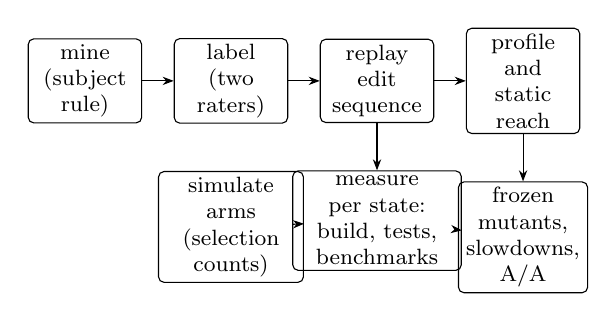
\begin{tikzpicture}[node distance=3mm and 4mm, every node/.style={font=\footnotesize},
  box/.style={draw, rounded corners=2pt, align=center, minimum height=7mm, inner sep=2pt, text width=13mm},
  arr/.style={-{Stealth[length=4pt]}}]
\node[box] (mine) {mine\\(subject rule)};
\node[box, right=of mine] (label) {label\\(two raters)};
\node[box, right=of label] (replay) {replay\\edit sequence};
\node[box, right=of replay] (prof) {profile and\\static reach};
\node[box, below=6mm of replay, text width=20mm] (measure) {measure per state:\\build, tests, benchmarks};
\node[box, below=6mm of prof, text width=15mm] (inject) {frozen mutants,\\slowdowns, A/A};
\node[box, below=6mm of label, text width=17mm] (arms) {simulate arms\\(selection counts)};
\draw[arr] (mine) -- (label); \draw[arr] (label) -- (replay); \draw[arr] (replay) -- (prof);
\draw[arr] (replay) -- (measure); \draw[arr] (prof) -- (inject); \draw[arr] (measure) -- (arms);
\draw[arr] (inject) -- (measure);
\end{tikzpicture}
\caption{Study pipeline. Mining, labelling and replay fix the edit sequence; profiles and static reach give benchmark coverage (RQ2); measured states and injected faults give cost, detection and power (RQ1, RQ3, RQ4).}
\label{fig:pipeline}
\end{figure}

\subsection{Subjects}
\textbf{networkx} is the main subject, chosen because it has an asv suite in its own repository, a pure-Python build (so build cost does not mask test and benchmark cost) and a recent history with many commits that describe themselves as performance changes. It has an asv suite of \NxBenchCases{} benchmark cases in \NxBenchFiles{} files and \NxNumTests{} tests.
\textbf{bottleneck}, a NumPy extension written in C from templates, is a contrast subject for build cost only, on \BnEdits{} replayed edits (states after an uncompilable replayed state are held out, Section~\ref{sec:lessons}).
\TODO{Table 2: subjects and edit counts. Add the E1 replication projects (3--4, chosen by the pre-registered order and attrition rule; candidates xarray, scikit-image, astropy, geopandas, shapely, pandas) with mined, labelled, true-optimization and profiled counts.}

\subsection{Edit mining, labelling and replay}
\textbf{Mining.} A commit qualifies if its subject matches a fixed regular expression for performance wording (\texttt{perf}, \texttt{speed up}, \texttt{faster}, \texttt{optimize}, \texttt{performance}, \texttt{vectorize}, \texttt{efficien}) and it changes package source.
For networkx we took the latest \NxMined{} qualifying commits before the study started (November 2026), in chronological order, without manual inclusion or exclusion; the number was fixed in advance to bound the cost of full validation at every state.
\TODO{Give the date span of the mined commits and their size (changed lines and functions per edit) in Table 2.}

\textbf{Unit of analysis and changed functions.} The unit is one replayed edit (one commit).
A Python function counts as changed if any removed or added line of the diff falls in its span, including its decorators and its qualified name inside classes and nested functions; added and deleted functions count, blank and comment-only lines do not.
Changed lines outside every function are module-level changes; they are excluded from coverage counts and expanded to all functions of the module by the selectors.
For bottleneck, C function definitions are found by a brace scan and template headers map to the Python-visible name.
\TODO{Validate the changed-function extraction against a hand check of a sample of edits and report the agreement.}

\textbf{Labelling.} Keyword mining is imprecise (Section~\ref{sec:lessons}), so every mined commit of four projects (\LabelRows{} rows, including the Q3 pilot projects of Appendix~\ref{app:q3}) was labelled from its subject, body and diff into three categories (optimization, not an optimization, unsure), using a frozen codebook whose question is whether the commit's main intent is to make existing code faster or use fewer resources without changing what it computes.
Two raters labelled all rows blind to benchmark reach, replay status and each other; a third agent, the adjudicator, decided the \LabelAdjudicated{} disagreements.
The raters were two LLM agents of the same model family; we treat this as a threat (Section~\ref{sec:threats}).
No human rater labelled the rows; the labels are agent labels throughout.
\TODO{Name the model and version of the raters and the adjudicator, and put the prompts in the artifact.}
Cohen's $\kappa$ over the three categories was \LabelKappa{} (\LabelAgree{} of \LabelRows{} rows agree).
The primary edit set for RQ2 is the commits both raters or the adjudicator labelled as optimizations; an earlier reading of the commit subjects alone is reported as a sensitivity set.
\TODO{Replication (E1): codebook v2 frozen before mining, agent-only labels as here, and held-out precision of the v2 mining rule.}

\textbf{Replay.} The mined commits are applied in order on top of the parent of the oldest one, giving a sequence of states $S_0, S_1, \dots$; \NxDropped{} of the \NxMined{} networkx commits did not apply and were dropped by rule, leaving \NxReplayed{} replayed edits (\NxStates{} states).
Of these, \NxAgentOpt{} are labelled optimizations by the agents and \NxManualOpt{} by the subject-only reading.
The replayed sequence is not a real optimizer session: consecutive edits are historical commits, not minutes-apart candidates of one agent.
Results that are per edit (RQ2, RQ3) do not depend on this; cost totals and the accumulation policy (RQ4) do.

\subsection{Arms}
Every arm validates every replayed edit.
\textbf{FULL} (A0) rebuilds from clean, runs all tests serially and all benchmarks.
\textbf{INC} (A1) builds incrementally.
\textbf{TESTMON} (A2) runs \texttt{pytest --testmon} unchanged, with its database carried across steps, as PerfAgent does~\cite{deng2026perfagent}.
\textbf{CHANGED-MODULE} (A3) runs the tests whose file name maps to a changed module.
\textbf{STATIC-BENCH} (A5) selects benchmarks whose static call-graph reach intersects the changed functions.
\textbf{A4} is our deterministic policy: function-level test selection over the changes accumulated since the last green full check, profile-based benchmark selection, and a full check triggered when an additive change score crosses a fixed threshold (a model-free variant of risk-mass batching~\cite{sayedsalehi2026riskaware}); its parameters were fixed before the runs.
Arms are also combined with periodic full checks every $k$ edits.
Test counts per arm come from real selections (testmon) or from the measured dependency map; seconds are estimated from per-test durations at $S_0$ and calibrated against measured end-to-end time.

\subsection{Coverage measures}
A benchmark case \emph{executes} an edit if its measured profile contains at least one function the edit changed (module-level lines excluded).
Profiles were recorded with \texttt{sys.monitoring} for all \NxBenchCases{} cases at $S_0$, during one call of each benchmark after its setup, so functions that run only in untimed setup or at import do not count as executed; this is a counting run, not a timing run.
\emph{Static reach} uses a conservative import and call graph from $S_0$.
An edit is \emph{unreached} if no case executes it.
Reach was taken at $S_0$ for all edits, not at each edit's parent.
\TODO{E1: profiles at each edit's parent for the replication projects, with the grouped profile runner validated against the networkx $S_0$ reach sets.}

\subsection{Oracles}
\textbf{Functional.} \MutantsFrozen{} mutants were frozen before any arm was configured, each placed in a function changed at its step; \MutantsKilled{} are killed by the full suite and form the functional fault set.
\textbf{Performance.} \NumSlowdowns{} synthetic slowdowns were frozen, each in a function changed at its step: nine call the function body twice and one replaces a set by a list for membership tests.
They are probes of detectability, not models of real regressions.
For each slowdown, a patched and an unpatched clone are measured interleaved (A/B), and a case is \emph{slower} under asv's rule: ratio of medians above \AsvFactor{} and a two-sided Mann-Whitney $p$ below \AsvAlpha~\cite{asvcommands}.
All primary verdicts use the exact Mann-Whitney test; re-testing all \RecomputeVerdicts{} verdicts with the exact test changed none of them (Section~\ref{sec:rq3}).
Within reach, each side has two processes with three values each, in three interleaved repeats; the profile-completeness check and the A/A control use five processes with three values per side and repeat.
A pre-registered noise floor additionally requires the ratio to exceed $1+3\sigma$, with $\sigma$ from a same-code A/A control.
The protocol also fixed strength bands for the regression set used to judge selection safety: a ``strong'' slowdown makes some case at least twice as slow, a ``moderate'' one between \BandModLo{} and \BandModHi\x.
\textbf{Test assumptions.} Mann-Whitney assumes independent samples; samples from one process are correlated, which makes $p$ optimistic, and repeating the oracle (Section~\ref{sec:rq3}) is the check. Wilson intervals assume independent trials; edits and slowdowns that share functions are not fully independent, so the intervals are optimistic.
\textbf{A/A control.} A frozen, seeded sample of \AACases{} cases (\AAAlgoCases{} of them from the heavy module) was run as $S_0$ against $S_0$ in two clones, with both run orders (ABBA), so every non-``same'' verdict is false.
Proportions are reported with Wilson 95\pct{} intervals.
\textbf{Exact test.} The rule we first implemented used scipy's default Mann-Whitney method, a normal approximation at these sample sizes, while asv uses an exact test; re-testing all \RecomputeVerdicts{} verdicts from their raw samples under the exact test changed \RecomputeChanged{} of them, and borderline $p$ values became smaller. All $p$ values in this paper are exact.
The smallest attainable two-sided exact $p$ is \MinPSixSix{} for six against six samples, above $\alpha=\AsvAlpha$ (Section~\ref{sec:lessons}), and \MinPFifteen{} for fifteen against fifteen.

\subsection{Platform and timing protocol}
All runs used one desktop machine (\texttt{Intel i5-12400F}, \TODO{core/thread and memory counts as macros}), WSL2 \texttt{Ubuntu 24.04}, \texttt{CPython 3.12}, with the package versions frozen in the artifact.
The CPU governor cannot be pinned under WSL2.
Timing runs start only when the machine is idle by a load gate (one-minute load average at most \LoadGate), and runs whose load exceeds the gate are labelled noisy and reported as such, not dropped.
Benchmarks use our asv-compatible runner with asv's default protocol for cost passes and more processes for verdicts.
Counts (reach, selections, detections) are machine-independent; wall times are reported as ranges over passes or as a median with its outliers named, never as single-pass point values.

\textbf{Ethics.} We analyse public open-source history and our own measurements; no personal data are analysed and no developers are named or assessed.

\section{RQ1: Where Does Per-Edit Validation Cost Go?}
\label{sec:rq1}

\paragraph*{Build and tests}
On networkx, the per-candidate build step (an editable install) takes a median of \NxBuildMedian\,s, \NxBuildShareTestsLo--\NxBuildShareTestsHi\pct{} of the serial test time.
The full suite of \NxNumTests{} tests passed at every state; serial test time per edit was \NxTestsLo--\NxTestsHi\,s across a first run and an idle re-run (median \NxTestsMedianClean\,s over the first run's clean-labelled states), of which about \NxPytestStartup\,s is pytest start-up and collection.
Over the base and the \NxReplayed{} replayed edits, serial tests alone took about \NxTestsSession\,s.

\paragraph*{Benchmarks}
One full benchmark pass (\NxBenchCases{} cases; our runner's cost protocol of two processes with three values each) took \NxBenchPassMin--\NxBenchPassMax\,s over \NxBenchPasses{} measured passes, with a median of about \NxBenchPassMedian\,s.
They are a dedicated pass at $S_0$, five unpatched sides of slowdown-oracle runs at later states, and three repeated passes at $S_0$ in one evening with machine telemetry, all with the same benchmark code and protocol; several were labelled noisy or concurrent.
Against about \NxBuildTests\,s for build plus serial tests, a benchmark pass costs at least about \NxBenchRatioTypical\x{} the rest of full validation even on the four fastest passes (\NxBenchPassMin--\NxBenchPassTypicalHi\,s), about \NxBenchRatioMedian\x{} at the median, and up to \NxBenchRatioHi\x{} (\NxBenchPassMax\,s) under drift, with the same code and protocol (Fig.~\ref{fig:cost}).
We lead with the lower bound because the claim is that benchmarks dominate, and because most passes were measured under load: by one uniform rule (a pass is noisy if any run exceeds the load gate or started without a passing gate), \PassesNoisy{} of the \NxBenchPasses{} passes are noisy, and the \PassesMeasured{} that is not is the unpatched side of an interleaved oracle run, so no pass is both clean and a dedicated full pass.
Pass times are run time only, excluding waits for the load gate.
The three repeated passes alone fell from \DriftEveningHi{} to \DriftEveningLo\,s (\DriftEveningRatio\x) within one evening, while their timing loops stayed at \DriftLoopsLo--\DriftLoopsHi\,s; almost all of the change was in one module's time outside the loops, and telemetry showed no covariate that moved with it.
Counting benchmarks, the build is below a fifth of a percent of a full validation at every measured pass.

\begin{figure}[t]
\centering
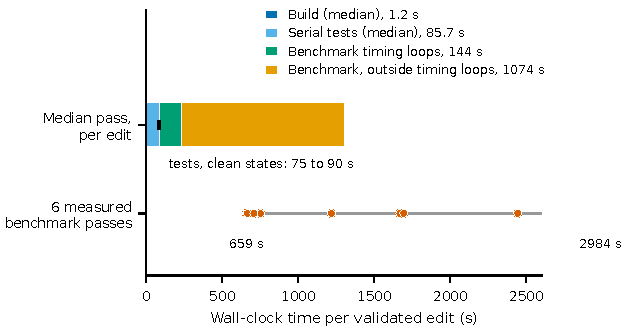
\includegraphics[width=\columnwidth]{figures/fig_cost.pdf}
\caption{Per-edit validation cost on networkx. Build and serial tests are medians with ranges over states; a full benchmark pass is split into time inside the timing loops and time outside them, over the measured passes (points). Single machine; wall times are ranges, not point values.}
\label{fig:cost}
\end{figure}

\paragraph*{Where benchmark time goes}
\NxAlgoShareLo--\NxAlgoShareHi\pct{} of a pass is spent in one module's \NxAlgoCases{} cases (\texttt{benchmark\_algorithms}), and \NxOutsideLoopsLo--\NxOutsideLoopsHi\pct{} of a pass lies outside the timing loops.
That module builds all its input graphs at import time, and asv's process isolation repeats the import for every case and process.
The timing loops themselves take only \NxLoopsLo--\NxLoopsHi\,s per pass.
If the setup were built once and reused, a pass would cost roughly its timing loops, about \NxSetupCachedLo--\NxSetupCachedHi\x{} build plus tests.
This is an estimate and a lower bound (it omits process start-up and warm-up), not a measurement.
\TODO{E5 (setup-cached pass): replace the estimate with a measured pass in which \texttt{benchmark\_algorithms}' graph construction moves into asv \texttt{setup\_cache} (or a cached fixture) in a patched copy of the suite; report loops, setup and total over at least three passes.}

Because the drift sits outside the timing loops, pass cost varies while verdicts on interleaved timed samples are shielded from slow drift (Appendix~\ref{app:drift}); it also means the setup, not the timing, is what a cached pass would remove.

\paragraph*{Contrast: a C extension}
On bottleneck, a clean build takes \BnBuildLo--\BnBuildHi\,s and the full suite (\BnNumTests{} tests) about \BnTests\,s, so the build is about \BnBuildShareLo--\BnBuildShareHi\pct{} of build plus tests.
Two full benchmark passes (\BnBenchCases{} cases, the same protocol, one state) took \BnBenchPassLo{} and \BnBenchPassHi\,s, so benchmarks cost about \BnBenchRatioLo--\BnBenchRatioHi\x{} build plus tests here too, and the build falls to about \BnBuildShareBenchLo--\BnBuildShareBenchHi\pct{} of a full validation.
Unlike networkx, the two passes agree closely, and about \BnLoopsShare\pct{} of the benchmark time is in the timing loops; we did not decompose the rest.
All bottleneck runs were labelled noisy, and the result covers one state.
\TODO{E4: R1 on one replication project with a cheap build and an asv suite (build, full tests, full benchmarks at 3--5 states, three passes each).}

\paragraph*{Answer to RQ1}
On networkx, benchmarks dominate per-edit validation cost, at least about \NxBenchRatioTypical\x{} build plus tests even on the fastest passes (about \NxBenchRatioMedian\x{} at the median), and most of their time lies outside the timing loops in one module, largely import-time setup by inspection; with that setup cached, the estimate drops to \NxSetupCachedLo--\NxSetupCachedHi\x, still the largest part but not by an order of magnitude.
Reducing the build saves almost nothing for this pure-Python project; reducing tests saves at most the test time of about a minute and a half per edit.
On bottleneck, a C-extension project with a non-trivial build, benchmarks also dominate, at about \BnBenchRatioLo--\BnBenchRatioHi\x{} build plus tests at one state.

\section{RQ2 and RQ3: Can the Benchmark Oracle See the Edit?}
\label{sec:oracle}

Whether a project's benchmarks can see a change to a function depends on three factors in turn.
The function must be \emph{executed} by some benchmark case (coverage, RQ2).
It must take a large enough \emph{share} of that case's time for a change to be \emph{visible} at the case level: a slowdown by a factor $f$ in a function with share $s$ changes the case by about $1+s(f-1)$, which is Amdahl's law applied to one benchmark case~\cite{amdahl1967validity}.
And the case-level effect must be \emph{detectable} above the measurement noise (power, RQ3).
None of these factors is new as a concept: Peass and Laaber and Leitner already separate uncovered changes from changes below the noise~\cite{reichelt2023peass,laaber2018evaluation}, and the share is an operationalisation of Amdahl's law that splits their ``below the noise'' case into a small effect and a noisy measurement.
What we add is a measurement of how often each factor bites for real optimization edits on one project.
Table~\ref{tab:oracle} lists the three factors per edit; the injected slowdowns at the end of this section test them.

\begin{table*}[t]
\caption{The benchmark oracle per agent-labelled optimization edit on networkx: number of benchmark cases whose $S_0$ profile executes a changed function; the largest share of a reaching case's time spent in the changed functions (cProfile at the edit's parent, approximate); and the expected case-level ratio $1+s(f-1)$ if the changed code were \PowFactorMid\x{} or \PowFactorHigh\x{} slower. Bold: above asv's factor of \AsvFactor{} at three decimals, so a flag is possible before noise is considered. ``--'': no case executes the edit.}
\label{tab:oracle}
\centering\footnotesize\setlength{\tabcolsep}{4pt}
% Generated by scripts/make_all.py (write_oracle_table). DO NOT EDIT.
\begin{tabular}{@{}rlrrrr@{}}
\toprule
Step & Changed function & Cases & Max share & Ratio at $1.2\times$ & Ratio at $2\times$ \\
\midrule
1 & \texttt{global\_parameters +1} & -- & -- & -- & -- \\
2 & \texttt{bidirectional\_dijkstra} & -- & -- & -- & -- \\
3 & \texttt{\_dijkstra\_multisource} & 8 & 0.864 & \textbf{1.173} & \textbf{1.864} \\
4 & \texttt{is\_connected +1} & 3 & 0.021 & 1.004 & 1.021 \\
5 & \texttt{\_single\_shortest\_path +2} & -- & -- & -- & -- \\
7 & \texttt{kruskal\_mst\_edges} & -- & -- & -- & -- \\
9 & \texttt{\_pagerank\_scipy +1} & 4 & 0.998 & \textbf{1.200} & \textbf{1.998} \\
10 & \texttt{\_build\_paths\_from\_predecessors} & 1 & 0.502 & 1.100 & \textbf{1.502} \\
11 & \texttt{DiGMState.\_\_init\_\_ +1} & -- & -- & -- & -- \\
12 & \texttt{edmonds\_karp\_impl +1} & -- & -- & -- & -- \\
14 & \texttt{\_build\_paths\_from\_predecessors} & 1 & 0.565 & \textbf{1.113} & \textbf{1.565} \\
15 & \texttt{lattice\_reference +1} & -- & -- & -- & -- \\
16 & \texttt{\_triangles\_and\_degree\_iter} & 4 & 0.999 & \textbf{1.200} & \textbf{1.999} \\
18 & \texttt{chain\_decomposition} & -- & -- & -- & -- \\
\bottomrule
\end{tabular}

\end{table*}
\TODO{Detectability per edit against each reaching case's measured noise floor needs $\sigma$ for those cases (only the flagged ones have it); add it as a column when available.}

\subsection{Executed: coverage of optimization edits (RQ2)}
\label{sec:rq2}

On networkx, for \BOneAgentUnreached{} of the \NxAgentOpt{} replayed optimization edits (\BOneAgentPct\pct, Wilson CI \ci{\BOneAgentLo}{\BOneAgentHi}), the measured profile of no benchmark case contains any function the edit changed (Fig.~\ref{fig:coverage}).
By static reach, \BOneAgentStatic{} of \NxAgentOpt{} are unreached (\BOneAgentStaticPct\pct, \ci{\BOneAgentStaticLo}{\BOneAgentStaticHi}).
With the earlier subject-only labels the counts are \BOneManualUnreached{} of \NxManualOpt{} (\BOneManualPct\pct, \ci{\BOneManualLo}{\BOneManualHi}) by profile and \BOneManualStatic{} of \NxManualOpt{} by static reach; over all \NxReplayed{} replayed edits they are \BOneAllUnreached{} and \BOneAllStatic{}.
The two label sets differ by one edit, which is unreached under both measures, so the reading does not depend on which of our two label sets is used.
Because every interval includes values below one half, we say that \emph{many} optimization edits on networkx are unreached, not most.

\begin{figure}[t]
\centering
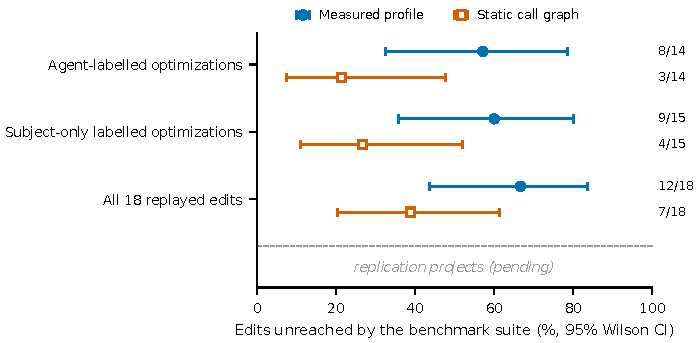
\includegraphics[width=\columnwidth]{figures/fig_coverage.pdf}
\caption{Share of replayed networkx edits that no benchmark executes, by measured profile and by static reach, with Wilson 95\pct{} intervals, for three edit sets. The replication rows are pending.}
\label{fig:coverage}
\end{figure}

\textbf{Reach at the base state.} Reach was measured with the $S_0$ suite and $S_0$ profiles.
A lookup of every changed function by qualified name found \ConstructUnreached{} edits unreached by construction: each has a changed function that exists at $S_0$, and all exist at their parent.
Profiles were still taken at $S_0$, not at each edit's parent, so a benchmark added upstream in between would be missed (Section~\ref{sec:threats}).
\TODO{Recompute with the upstream suite and profiles at each edit's parent, as the replication protocol does.}

\textbf{Static reach is not a bound.} Static reach leaves fewer edits unreached than the measured profile on every edit set, because the heavy benchmark module imports most of the package and a static graph connects it to functions it never calls; from an old base it can also miss functions added later (Appendix~\ref{app:q3}).
The motivating edit (step~2) is an example: static reach connects all \NxBenchCases{} cases to \texttt{bidirectional\_dijkstra}, and no profile executes it.
We therefore count reach by measured profile only.

\TODO{E1 (B1 replication): to meet the bar for the full paper, at least four to five projects and fifty to sixty labelled true optimizations pooled, with profiles at each edit's parent; per-project and pooled unreached shares with Wilson CIs as forest-plot rows in Fig.~\ref{fig:coverage}; attrition per the pre-registered rule; and the thesis restated or reframed by the pre-registered decision rule.}

\subsection{Visible: the changed function's share of a case}
\label{sec:share}

For the injected slowdowns, we estimated the share of each reaching case's time spent in the slowed function with cProfile at the slowdown's state (unpatched), as the function's inclusive time over the case's profiled time.
cProfile overhead inflates call-heavy code, so the shares are approximate.
For a slowdown that calls the function body twice, the expected case-level ratio is about one plus the share.

\textbf{A share miss.} \#3 (\texttt{is\_connected}) is executed by three profiled cases of the heavy module but takes only about \ShareThreeLo--\ShareThreeHi{} of their time, so doubling it should change them by a ratio of about \ExpThree; the observed ratios stayed near one.
asv's ratio condition (above \AsvFactor) can never flag such a change, however many samples are taken.
\#3 is therefore a miss of a diluted effect: executed by a benchmark is not the same as visible to it.

\textbf{Detections match the share.} For \#2 the share is \ShareTwoLo--\ShareTwoHi, which predicts ratios close to the observed \SlowTwoRatioLo--\SlowTwoRatioHi.
For \#8 the share is \ShareEight, but its slowdown changes one membership test inside the function rather than doubling the body, so one plus the share does not predict its ratio.
\textbf{Per optimization edit.} We computed the same share for every agent-labelled optimization edit, at the edit's parent state, as the largest share of any reaching case's time spent in the changed functions (Table~\ref{tab:oracle}).
Of the \NxAgentOpt{} edits, \BOneAgentUnreached{} are executed by no benchmark; one (step~4) is executed but diluted, with a share of \EditShareDiluted, so even a doubling of its code would move its benchmarks by about two percent; and the others have large shares (\EditShareBigLo--\EditShareBigHi).
If the changed code were \PowFactorMid\x{} slower, at most \EditsClearMid{} of the \NxAgentOpt{} edits would move a benchmark past asv's factor at all, before noise is considered; one more (step~10) sits at the factor, and because the cProfile share is approximate (to about a hundredth), it cannot be classified either way. At \PowFactorHigh\x, \EditsClearHigh{} would.
These are expected effects from approximate shares, not detections; the noise floor below decides which of them a run would flag.

\subsection{Detectable: noise and power (RQ3)}
\label{sec:rq3}

In the A/A control, asv's rule gave \AAFalse{} false verdicts in \AAComparisons{} per-repeat comparisons (Wilson upper bound \AAUpper\pct); the \AAComparisons{} comparisons are the same \AACases{} cases twice, so the bound is optimistic.
The noise sits near the threshold: some cases passed the $p$ condition and stayed ``same'' only on the ratio condition, and under a fixed run order one case reached a ratio of \AAMaxSameRatio{} without passing the $p$ condition.
\textbf{The pre-registered floor.} For every case with a slower verdict we ran an A/A at the verdict's own state and protocol, \SigmaRepeats{} repeats with the order rotated, and applied the pre-registered rule: a verdict survives if its ratio exceeds $1+3\sigma$, with $\sigma$ the standard deviation of the per-repeat A/A ratios.
Only \#2's on-target verdicts survive (all \SlowTwoCases{} cases, also under a bootstrap $\sigma$).
\#8's case has a floor of \FloorEight, so it cannot detect a slowdown of the size injected; its own A/A run even returned ``slower'' (pooled ratio \EightAAPooled), so its original verdict is indistinguishable from noise.
\#1's off-target case (floor \FloorOne) and the profile-completeness flag for \#9 (\SlowNineRatio\x{} against a floor of \FloorNine) do not survive either.
With five repeats, each $\sigma$ has four degrees of freedom, so every floor is uncertain; \#2's margin is large, while \#9 sits at its floor.
\TODO{E2 remainder: $\sigma$ for the other benchmark cases (none outside the flagged ones has it), and a larger heavy-module A/A sample of at least ten seeded cases.}

\textbf{Power at the verdict design.} We bootstrapped detection probability from the A/A samples at the verdict design (\VerdictSamples{} pooled samples per side, exact test) under asv's rule plus the pre-registered floor.
At a slowdown of \PowFactorMid\x, the median detection probability is \PowDesignAllMid{} over all A/A cases, but only \PowDesignAlgoMid{} for the \AAAlgoCases{} sampled cases of the heavy module (\PowDesignAlgoMidBoot{} with a bootstrap $\sigma$; \PowDesignAlgoMidNoFloor{} without the floor); at \PowFactorOneFive\x{} it is \PowDesignAlgoOneFive{} and at \PowFactorHigh\x{} \PowDesignAlgoTwo{} for those cases.
So once the floor applies, the module that holds most of the cost reliably detects only slowdowns of about \PowFactorOneFive\x{} or more.
This rests on \AAAlgoCases{} of its \NxAlgoCases{} cases and on $\sigma$ from two A/A repeats, and the bootstrap ignores the structure between processes and repeats, so the values are optimistic and indicative, not a module-wide estimate.
Fig.~\ref{fig:power} shows the earlier bootstrap at the A/A design (fifteen samples per side, no floor), which gives \PowAllOneTwo{} and \PowAlgoOneTwo{} at \PowFactorMid.

\begin{figure}[t]
\centering
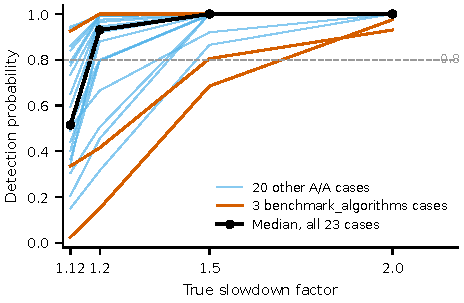
\includegraphics[width=\columnwidth]{figures/fig_power.pdf}
\caption{Bootstrap detection probability of asv's rule under the exact Mann-Whitney test, by slowdown factor, for the A/A cases on networkx. The heavy-module curve rests on three sampled cases.}
\label{fig:power}
\end{figure}

\subsection{Injected slowdowns as the test}
\label{sec:slowdowns}

\textbf{Pre-registered primary result.} Regression safety of reduced benchmark selection is \emph{not measurable} on networkx with the frozen slowdown set: no slowdown was detected on target within the pre-registered strength bands, so the regression set that selection arms were to be judged on is empty.
This is partly a consequence of the bands: the on-target ratios of \#2 (\SlowTwoRatioLo--\SlowTwoRatioHi\x) fall in the gap between the moderate band's upper end (\BandModHi\x) and the strong band (twofold), and \#8 (\SlowEightRatio\x) falls below the moderate band.

\textbf{Detection.} Fig.~\ref{fig:slowdowns} classifies the \NumSlowdowns{} slowdowns.
One rule decides all flags: a flag counts as a detection only if the flagged case executes the slowed function in its profile; other flags are reported as off target.
Within reach, each verdict compares \VerdictSamples{} pooled samples per side.
Slowdown \#$k$ sits in the function changed at one replay step: \#0--\#5 at steps one to six and \#6--\#9 at steps eight to eleven.
Under asv's rule the full suite flags \SlowDetClassified{} slowdowns (Wilson \ci{\SlowDetClassLo}{\SlowDetClassHi}), \SlowDetOnTarget{} of them on target (\ci{\SlowDetOnTargetLo}{\SlowDetOnTargetHi}); above the pre-registered noise floor it detects \FloorDetect{} (\ci{\FloorDetectLo}{\FloorDetectHi}).
\#2 (\texttt{\_dijkstra\_multisource}) is flagged by all \SlowTwoCases{} profiled cases at \SlowTwoRatioLo--\SlowTwoRatioHi\x, far above their floors; \#8 (\texttt{\_build\_paths\_from\_predecessors}) is flagged by its one profiled case at \SlowEightRatio\x, below that case's floor of \FloorEight.
\#1's only flag (\SlowOneRatio\x, exact $p=\SlowOneExactP$) is on a case that never executes \texttt{bidirectional\_dijkstra}, whose body is the only code the patch changes; we classify it as an off-target flag, and it does not pass its floor either.
Across the oracle, \OffTargetVerdictable{} off-target comparisons could yield a verdict (plus fifty spot-check comparisons that cannot, \OffTargetComparisons{} in all); \OffTargetObserved{} of them gave a non-``same'' verdict.
At the nominal $\alpha=\AsvAlpha$ about \OffTargetExpected{} would be expected, but the null rate of the joint rule is not calibrated here (samples within a process are correlated, the comparisons share cases, and the ratio condition and the discreteness of the exact test pull the other way), so we report the off-target flags descriptively rather than as consistent with chance; the repeat below found off-target flips on about \TwoFlipPct\pct{} of cases in this fixed-directory design.

\begin{figure}[t]
\centering
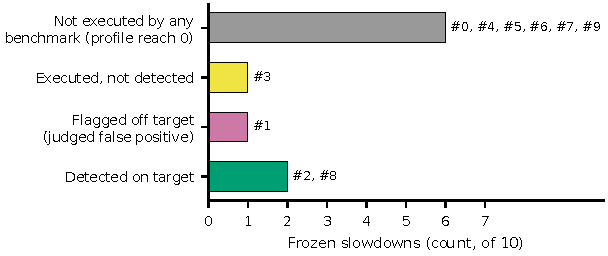
\includegraphics[width=\columnwidth]{figures/fig_slowdowns.pdf}
\caption{The frozen slowdowns on networkx by outcome under the full suite: not executed by any benchmark in its measured profile (coverage miss), executed but not detected, detected on target, and flagged off target.}
\label{fig:slowdowns}
\end{figure}

\textbf{Misses by factor.} Static reach does not separate these slowdowns: the $S_0$ static call graph connects all \NxBenchCases{} cases to each of \#1--\#4 and \#8, so we classify by measured profile only (no case for \#1 and \#4, three for \#3, \SlowTwoCases{} for \#2, one for \#8).
We count a slowdown as missed when it is not detected on target, so \#1, flagged only off target, is missed.
Of the \SlowUndetected{} missed slowdowns, \SlowUnreachedProfile{} lie in functions that no measured profile executes (\SlowMissedUnreached{} of them unreached by static reach as well, plus \#1 and \#4), and \#3 is the share miss above.
Because the slowdowns were placed in functions changed at their step, these counts follow from the reach of those functions; they check the profiles and the share argument, and are not an independent rate.
Under the pre-registered floor, \#8 is missed as well, and it is the one power miss in this set: its slowed function takes about half of its case's time, but that case's noise is too high (floor \FloorEight) for the effect to be distinguished.

\textbf{What this says about selection.} On this protocol, no selection among these benchmark cases can detect a slowdown that running all of them misses; with the same time budget, a selected subset could be run with more repetitions and gain power, which we did not test.
A check of the profiles' completeness (Appendix~\ref{app:completeness}) found one flag outside the measured reach, which neither passes its noise floor nor reproduced in a post-hoc re-check.

\textbf{Repeatability.} We repeated the oracle on the verdict-relevant cases of \#1, \#2, \#3 and \#8 at each slowdown's own state, with four repeats in alternating order (\RepSamples{} pooled samples per side, \RepRuns{} runs).
\RepAgree{} of \RepTotal{} verdicts agree with the original.
\#2's on-target verdicts repeat on all \SlowTwoCases{} cases at \RepTwoLo--\RepTwoHi\x.
The two off-target flags (\#1, and \#2's off-target case) do not repeat and are now ``same'', consistent with noise.
\#8 is again ``slower'' pooled (\RepEightRatio\x), but each order-balanced pair is ``same'', the ratio is far below its floor, and the same case's A/A also returned ``slower'', so the agreement carries no evidence of a real effect.
\#3 is ``same'' on all three cases, which is no evidence of an effect at this protocol; on one case a moderate effect is not excluded.
Detection above the floor therefore stays at \FloorDetect{} of \NumSlowdowns, a result the repeat checks only for \#1, \#2, \#3 and \#8.
\#1's block was interrupted by a time cap and resumed hours later, so its second order-balanced pair mixes runs from two sessions; its ratio matches the first pair.
A second tier repeated the off-target cases of all five reached slowdowns with two order-balanced repeats; for \#2, \#3 and \#4 each side kept one clone directory, as in the original oracle.
Of \TwoTotal{} off-target verdicts, \TwoAgree{} again read ``same'' and \TwoFlips{} (\TwoFlipPct\pct, Wilson \ci{\TwoFlipLo}{\TwoFlipHi}, too narrow because cases share runs) became non-``same'', against about \TwoExpected{} expected at the nominal level; that nominal level assumes exchangeable samples, which pooled runs from few processes are not.
\TwoFaster{} of these flips are ``faster'', which a patch that only adds work cannot cause.
In every A/B run, including the original oracle, the unpatched side ran in one clone directory and the patched side in another, so the edit and the clone directory are confounded.

\textbf{Identical code.} To test whether such flips need an edit at all, we ran the same tier-2 cases and design with identical, unpatched code in the two clone directories.
\DirAANonSame{} of \DirAATotal{} cases still returned a non-``same'' verdict (\DirAAPct\pct, Wilson \ci{\DirAALo}{\DirAAHi}), a rate the intervals cannot distinguish from the \TwoFlipPct\pct{} with the patches, and only \DirAARecur{} of the \DirAARecurN{} earlier flips at that state recurred.
So the off-target flips need no effect of the edit.
This control also kept one directory per side, so for \#8 and \#1 we swapped the directories between the two repeats, balancing the edit across directories (and, with it, run order).
The swap did not remove the flips: \SwapFlips{} of \SwapTotal{} off-target verdicts (\SwapPct\pct) became non-``same'', and none reversed its sign when the directories swapped, so a directory effect alone does not produce them.
Nor do they show a stable effect of the edit: of the \CrossNightN{} \#8 cases that could be compared with an earlier night under the same setup, only \CrossNightAgree{} reproduced, and sign consistency across repeats is expected after selecting on a small pooled $p$ (the identical-code flips kept their sign too).
Their cause, per-night variation, an anti-conservative test on correlated samples, or an effect specific to a few sensitive cases (one \texttt{connected\_components} case flags under two unrelated slowdowns), is unresolved, and we could not test machine load.
In this design, then, single A/B verdicts up to about \DirAAMaxDev\x{} in either direction, the largest deviation seen with identical code, are not evidence of an edit effect; at the tier-2 sample size, about \DirAAFalsePerComp{} false changes (\DirAAFalseLo--\DirAAFalseHi) are expected per comparison of all \NxBenchCases{} cases, assuming independent cases.
This covers \#8 (\SlowEightRatio--\RepEightRatio\x), all off-target flags and the profile-completeness flag.
\#2's on-target ratios (\RepTwoLo--\RepTwoHi\x) lie well above it, cleared their own noise floors and repeated, so \#2 stands as the one detection.
The swapped run repeated only off-target cases, so \#8's on-target verdict was not re-tested with swapped directories.

\paragraph*{Answers to RQ2 and RQ3}
On networkx, the project's own benchmarks execute none of the changed functions for many optimization edits (\BOneAgentUnreached{} of \NxAgentOpt{}, CI \ci{\BOneAgentLo}{\BOneAgentHi}); for those, full benchmarking cannot confirm the speed-up or see a slowdown in the changed functions, as far as one profile shows (RQ2).
Where a benchmark does execute the changed code, its share and the noise decide (RQ3): above the pre-registered floor the full suite detected \FloorDetect{} of \NumSlowdowns{} injected slowdowns, the one whose function dominates its cases; one slowdown was hidden by a small share and one by noise; and per edit, at most \EditsClearMid{} of the \NxAgentOpt{} optimization edits could show a \PowFactorMid\x{} slowdown of their changed code at all.

\section{RQ4: What Do Deterministic Reductions Save?}
\label{sec:rq4}

Table~\ref{tab:arms} lists the arms over the \NxReplayed{} replayed networkx edits.
Benchmarks are excluded from these totals; RQ1 shows that they would dominate them.

\begin{table}[t]
\caption{Arms over the replayed networkx edits: tests run, estimated and measured end-to-end test cost (build plus tests plus start-up, no benchmarks), and misses of the frozen functional mutants (Wilson 95\pct{} CI of the miss rate). Estimated seconds come from per-test durations and are comparable across arms; measured seconds are single runs under different load and are not comparable with the estimates. INC equals FULL in tests run; STATIC-BENCH equals TESTMON in tests and differs only in benchmarks.}
\label{tab:arms}
\centering\footnotesize\setlength{\tabcolsep}{4pt}
\begin{tabular}{@{}lrrrl@{}}
\toprule
Arm & Tests & Est.\ s & Meas.\ s & Missed (CI) \\
\midrule
FULL (A0) & \TestsRunFull & \EstFull & \FullMeasured & \MutantsNone/\MutantsKilled{} \ci{\MutantsNone}{\ZeroMissHi} \\
TESTMON (A2) & \TestsRunTestmon & \EstTestmon & \TestmonMeasured & \MutantsNone/\MutantsKilled{} \ci{\MutantsNone}{\ZeroMissHi} \\
CHANGED-MOD.\ (A3) & \TestsRunAThree & \EstAThree & -- & \AThreeMissed/\MutantsKilled{} \ci{\AThreeMissLo}{\AThreeMissHi} \\
A4 (ours) & \TestsRunAFour & \EstAFour & -- & \MutantsNone/\MutantsKilled{} \ci{\MutantsNone}{\ZeroMissHi} \\
\bottomrule
\end{tabular}
\end{table}

\paragraph*{Incremental build}
For networkx, an incremental build saves almost nothing: the clean build is \NxBuildShareTestsLo--\NxBuildShareTestsHi\pct{} of the test time.
For bottleneck the build is a larger share of build plus tests (Section~\ref{sec:rq1}), but small once benchmarks count.
We report it as negligible for this project, not as a saving.

\paragraph*{Test selection, end to end}
pytest-testmon, unchanged, took \TestmonMeasured\,s over the replayed sequence against \FullMeasured\,s for full serial tests and builds, and \FullIdle\,s in the idle re-run: \TestmonRatioLo--\TestmonRatioHi\x{} cheaper.
Counting only the seconds of the tests run would suggest \TestSecRatio\x{} (\TestmonTestSec{} against \FullTestSec\,s).
The difference is pytest start-up, paid per step, and testmon's own analysis; its first run, which builds the database, took \TestmonDB\,s against \TestmonDBPlain\,s for a plain run.
The testmon measurement ran concurrently with other work and the full run includes one noisy state, so the ratio is a range.
On the worked example of step~10, test time falls from about \WorkedTestsBefore\,s to \WorkedTestsAfter\,s, about \WorkedRatio\x, because start-up remains.
Reductions in tests run, as optimizers report them (PerfAgent reports large shares of tests skipped~\cite{deng2026perfagent}), are therefore not proportional reductions in validation time: on networkx, a \TestSecRatio\x{} cut in test-seconds became \TestmonRatioLo--\TestmonRatioHi\x{} end to end, in one run under mixed load.

\paragraph*{Functional safety}
Every arm except CHANGED-MODULE caught all \MutantsKilled{} frozen mutants at the step that introduced them.
CHANGED-MODULE missed \AThreeMissed: in both, the killing tests live in a test file whose name does not match the module.
With a full check every three or every five edits, both are caught one or two steps later.
Because the mutants sit in the edited functions, every arm that selects by dependency catches them by construction; this fault model cannot rank selection rules, only show that the cheap arm is not obviously unsafe.

\paragraph*{Our accumulated-change policy (negative result)}
A4 selects tests over the change accumulated since its last full check and triggers a full check when an additive change score crosses a fixed threshold.
On this sequence it behaved like periodic full checks every \AFourK{} edits or so, and it bought no extra detection: plain testmon catches the same mutants at about half its estimated cost (\EstTestmon{} against \EstAFour\,s).
The accumulation null, the collapse of its benchmark selection and the batching comparison are in Appendix~\ref{app:a4}.

\paragraph*{Answer to RQ4}
On networkx, existing test selection saves \TestmonRatioLo--\TestmonRatioHi\x{} of test-validation time end to end with no functional miss on the frozen mutants, and incremental builds save almost nothing.
Our deterministic accumulated-change policy adds nothing measurable under this fault model.
Neither touches the benchmark cost of RQ1.

\section{Discussion}
\label{sec:discussion}

\paragraph*{What an optimizer accepts}
An optimizer that accepts an edit when ``tests pass and benchmarks are not slower'' relies on an oracle that, on networkx, executes none of the changed functions for \BOneAgentUnreached{} of \NxAgentOpt{} optimization edits, and that, where it does execute them, missed one slowdown because the function was a small part of the benchmark and another because the benchmark's noise was too high, and where at most \EditsClearMid{} of the \NxAgentOpt{} optimization edits could show a \PowFactorMid\x{} slowdown of their changed code at all.
For such edits the benchmark verdict ``not slower'' carries no information about the changed functions, as far as one profile shows, and a claimed speed-up is unconfirmed.
Reducing build and test work, which existing tools already do, leaves this untouched; it shortens the cheap part of validation.
\TODO{Restate with the pooled replication share (E1); if replication fails, restate as ``depends on suite design'' and keep networkx and bottleneck as the two cases.}

\paragraph*{Recommendations}
For optimization pipelines and benchmark harnesses that use a project's benchmarks as the performance oracle, the results suggest three practices.
(1)~Report, for every accepted edit, whether any benchmark executes a changed function and what share of that benchmark's time the function takes, so that ``not slower'' is read only where it means something.
(2)~Where no benchmark reaches the edit, time the unit tests that do reach it, as SWE-Perf does for its tasks~\cite{he2025sweperf}, as a deterministic fallback oracle, with a measured noise floor.
(3)~Look at time outside the timing loops before selecting benchmarks: on networkx it is the largest single cost, and by inspection it is mostly import-time setup that caching could remove, whereas selection only scales it down; how much caching saves is not yet measured.
\TODO{Unit-test fallback (no new run): count how many of the unreached optimizations are executed by at least one unit test, from the existing networkx dependency map; this is the deterministic baseline that generated workloads must beat.}

\paragraph*{Suite design as a hypothesis}
The networkx suite is organized by graph class and algorithm family, with one module holding most algorithm benchmarks.
bottleneck's suite, by contrast, names its functions directly; a source reading shows that even there one benchmark of \texttt{nanmax} calls \texttt{nanmin}, so code specific to \texttt{nanmax} is never benchmarked.
We hypothesize that whether benchmarks see optimization edits depends on how the suite is written; the replication across projects is designed to test this.

\paragraph*{Towards targeted workloads}
Unreached and low-share edits are where generated, edit-specific workloads could help.
This study sets the deterministic baseline that such generation must beat; generating workloads, with or without LLMs, is outside its scope.

\subsection{Lessons for measuring this problem}
\label{sec:lessons}

\paragraph*{Keyword mining of ``performance'' commits is imprecise}
The precision of the subject rule, against the adjudicated agent labels, was \PrecNx/\PrecNxN{} on networkx, \PrecBn/\PrecBnN{} on bottleneck, \PrecGp/\PrecGpN{} on geopandas and \PrecPv/\PrecPvN{} on pvlib-python (pooled \PrecPooled/\PrecPooledN, \PrecPooledPct\pct, \ci{\PrecPooledLo}{\PrecPooledHi}).
On pvlib-python the word stem \texttt{efficien} matches ``coefficient'' and ``efficiency'', and \texttt{optimi[sz]} matches \texttt{scipy.optimize}.
Counts of ``optimization commits'' that rest on keyword hits alone can therefore mislead; every count in this paper uses labelled optimizations.

\paragraph*{Small spot checks have no power by construction}
A comparison of six against six samples cannot reach $p<\AsvAlpha$ with a two-sided Mann-Whitney test: the smallest attainable $p$ is \MinPSixSix.
Our first out-of-reach spot check had this size; its ``no slower case'' result held by construction and was withdrawn.
Any asv-style check with one process and few values per side has the same property.

\paragraph*{Two smaller lessons}
Mapping the same networkx state twice with identical settings attributed \CSevenFuncs{} of \CSevenTotal{} functions (\CSevenPct\pct) to different test sets, so function-level dependency data needs a repeat run before it is trusted.
On bottleneck, a replayed state that did not compile still passed \HOnePassed{} tests on the parent's compiled extensions (the clean build failed); it is a replay artefact, but it shows that a validation harness must reject a failed build whatever the tests say.

\section{Threats to Validity}
\label{sec:threats}

We follow the classification of Wohlin et al.~\cite{wohlin2024experimentation} and list only threats specific to this study~\cite{verdecchia2023threats}.

\subsection{Construct validity}
\textbf{Executed is not able to detect.} RQ2 counts whether a benchmark executes a changed function~\cite{sjoberg2022construct}. Execution is necessary for detection, not sufficient: a benchmark may run the function on a trivial path. RQ2 is therefore an upper bound on what the suite can detect, and RQ3 measures the power side separately. The bias of RQ2 is towards \emph{fewer} undetectable edits than there are.
\textbf{What counts as an optimization edit.} The edit set depends on labels. All labels come from LLM agents: two blind raters and an adjudicator, all of the same model family; no human labelled the rows. Their agreement ($\kappa=\LabelKappa$) therefore overstates independent agreement, because raters of one model share its errors. One adjudicated label (a geopandas commit) cited details that the labelling sheet's truncated diff did not show; checked against the full commit diff, most cited details are present and one is not, and the label stands. The unreached count changes by one edit between the agent labels and an earlier reading of the commit subjects alone, and the interval is reported for both; neither set is human-validated.
\textbf{Synthetic slowdowns.} Calling a function body twice is a controlled probe of detectability, not a model of real regressions; it usually produces a large slowdown in the slowed function, so detection rates of moderate real regressions are likely lower than ours.
\textbf{Profiles at one state, one call.} Reach was profiled with the $S_0$ suite at $S_0$ for all edits, one call per case, not at each edit's parent. A lookup by qualified name found \ConstructUnreached{} edits unreached by construction (Section~\ref{sec:rq2}), but a benchmark added upstream between $S_0$ and an edit would be missed, which biases the unreached count upward. A re-profile reproduced the reach sets it covered, but profiles are samples of reach (Section~\ref{sec:lessons}).
\textbf{Time shares are approximate.} The share of a case's time spent in a slowed function comes from cProfile, whose overhead inflates call-heavy code; we use it only to classify misses, where the shares are far from the decision threshold.

\subsection{Internal validity}
\textbf{Machine noise and drift.} All timings come from one machine under WSL2, where the governor cannot be pinned; per-process setup cost drifted during the day for unknown reasons. Verdicts compare interleaved samples, which shields ratios from slow drift but not from changes in variance; cost is reported as ranges over passes. Some runs exceeded the load gate and are labelled noisy; none was silently dropped. \TODO{Drift passes with telemetry (E6) and, if granted, a pinned native-Linux machine for E2, E3 and E5.}
\textbf{Post-hoc analyses and deviations.} Several analyses were added after seeing data, and several protocol steps were not run as pre-registered; they are listed in Section~\ref{sec:deviations} and labelled where used. The primary pre-registered results (regression safety not measurable; the profile-completeness flag for \#9; the accumulation null) are reported unchanged.
\textbf{Concurrent work.} Other jobs on the same machine overlapped some runs; overlaps are logged per run, and those runs carry a noisy or concurrent label.
\textbf{Clone directory confounded with the edit.} Every A/B comparison ran the unpatched side in one clone directory and the patched side in another, so a verdict cannot separate the patch from differences between the clones; a repeat found off-target flips of both signs on about \TwoFlipPct\pct{} of cases. This biases off-target verdicts towards false flags; the on-target detection of \#2, which repeats at a ratio far above its noise floor, is unlikely to be explained by it. Swapping or rotating the directories between sides would remove the confound.

\subsection{External validity}
\textbf{One project for the main results.} RQ2 and RQ3 rest on networkx, with \NxAgentOpt{} optimization edits; the coverage interval is wide (\ci{\BOneAgentLo}{\BOneAgentHi}). Our static pilot on other projects is not evidence (Appendix~\ref{app:q3}). Every result is stated for networkx until the replication lands. \TODO{E1 replication on 3--4 projects; per-project and pooled results.}
\textbf{Replayed commits stand in for a session.} Historical commits are larger and further apart than an optimizer's candidates. Per-edit results (coverage, power) do not depend on the session model; cost totals and the accumulation policy do.
\textbf{Python, asv, small builds.} The build results hold for pure-Python and small C-extension builds; we did not study a project with a heavy build.

\subsection{Conclusion validity}
\textbf{Small samples.} Proportions over \NxAgentOpt{} edits, \NumSlowdowns{} slowdowns and \MutantsKilled{} mutants have wide intervals, which we report everywhere; ``no miss'' means a miss rate below the interval's upper bound, not safety.
\textbf{Multiplicity.} The oracle made \OffTargetVerdictable{} off-target comparisons that can yield a verdict at $\alpha=\AsvAlpha$; about \OffTargetExpected{} false verdicts would be expected at the nominal level and \OffTargetObserved{} were observed, but the null rate of the joint rule is not calibrated here, and samples from one process are not independent, which makes Mann-Whitney $p$ optimistic. A repeat of \TwoTotal{} off-target comparisons produced \TwoFlips{} new non-``same'' verdicts (about \TwoFlipPct\pct{} in this fixed-directory design, source unresolved), so off-target and small on-target verdicts such as \#8 cannot be read individually. Both original off-target flags were first judged noise by a reach argument and did not repeat.
\textbf{Power of the A/A control.} \AAComparisons{} comparisons of \AACases{} cases cannot separate a small false-verdict rate from zero, and the heavy-module estimate rests on \AAAlgoCases{} cases. \TODO{E2 sigma.}
\textbf{Exact test.} Verdicts were first computed with a normal approximation; re-testing all of them exactly changed none.

\subsection{Reliability and research process}
\label{sec:deviations}
\textbf{Artifacts.} Frozen inputs carry hashes; raw files record the state and harness version; the paper's numbers and figures are generated from the raw files by a script that fails if they disagree. One raw file (the A/A $\sigma$ estimates) lacks its metadata block. \TODO{Artifact package and DOI.}
\textbf{Deviations from the pre-registration.} (1) The noise floor $1+3\sigma$ was applied to every flagged verdict, with $\sigma$ from five A/A repeats at each verdict's own state rather than at $S_0$ as planned; the other benchmark cases still have no $\sigma$. (2) The first out-of-reach spot check had no power and was replaced by a powered profile-completeness check. (3) The labelling rule for noisy test runs was written after the first look at two slow states. (4) Edit labels were added after mining, and the mining rule was not changed for this study. (5) A per-arm regression simulation was not run. \TODO{Full deviation table in the artifact; update after E2.}
\textbf{AI assistance.} The selection and validation rules contain no learned or LLM component; the commit labels that define the RQ2 edit set were produced by LLM agents (construct validity, above). Large parts of the harness, the analysis scripts and the text were also produced with AI assistance. \TODO{Disclose per the chosen venue's policy; the authors re-derive every headline number from the raw files before submission.}

\section{Conclusion}
\label{sec:conclusion}

We set out to make per-edit validation of code optimizations cheaper with reduced builds and reduced test and benchmark selection, using deterministic rules.
On networkx, the expensive part of validation is the benchmarks, at about \NxBenchRatioMedian\x{} the build plus tests for the median pass, mostly outside the timing loops; existing test selection saves \TestmonRatioLo--\TestmonRatioHi\x{} of the rest end to end, and our accumulated-change policy adds nothing measurable.
In the base-state profiles, the same benchmarks execute none of the changed functions for \BOneAgentUnreached{} of \NxAgentOpt{} optimization edits, and they detect \FloorDetect{} of \NumSlowdowns{} injected slowdowns on target above the pre-registered noise floor (\SlowDetOnTarget{} by asv's rule alone); where they do execute an edit, the changed code's share of their time means that at most \EditsClearMid{} of the \NxAgentOpt{} edits could show a \PowFactorMid\x{} slowdown at all.
On this project, the limiting part of per-edit validation was the performance oracle, not build or test cost.
\TODO{Final sentence after E1: whether this holds across the replication projects, and the per-project range.}


\bibliographystyle{IEEEtran}
\bibliography{refs}

\appendices
\section{The A4 policy and batching comparators}
\label{app:a4}
A4 combines (a) function-level test selection over the change accumulated since the last green full check, (b) benchmark selection by stored profiles refreshed at each full check, and (c) a full check when an additive score reaches the threshold $T=\AFourT$, plus a final full check.
The score is the number of accumulated changed functions (a module-level edit counts every function of its module) plus a fixed penalty for each distinct C header edit and each native fallback since the last green full check.
It targets faults that stay latent until a later edit makes them observable, which a per-edit selection over the current change alone could miss.
All parameters were fixed before the runs and not tuned.
\textbf{Behaviour.} On the replayed networkx sequence A4 fired \AFourChecks{} full checks, each caused by an edit at module level; its estimated cost (\EstAFour\,s) lies between testmon with a full check every five edits (\EstTestmonKFive\,s) and every three (\EstTestmonKThree\,s).
\textbf{Accumulation null.} Accumulation added \AccumExtraRuns{} test runs and found nothing, as pre-registered: \LatentFound{} of the \MutantsSurvive{} mutants that survive the full suite become detectable at a later state, so the class of faults that accumulation targets is empty on networkx.
\textbf{Ablations.} Removing the order-dependence rule, the accumulation, or the profile rule leaves functional detection unchanged on the frozen mutants; removing accumulation removes \AccumExtraRuns{} test runs.
\textbf{Benchmark selection collapses.} Because profiles exist only at $S_0$, the rule that profiles must not be older than the last checkpoint marks every profile unknown after the first full check, and the conservative default selects all benchmarks. A labelled variant that violates this rule by reusing $S_0$ profiles selects \BTwoVariant{} cases in total, against \BTwoStatic{} for static reach and \BTwoFull{} for running everything.
\textbf{Batching at matched cost.} Against pure batching with a fixed cap or an additive budget, interpolated to A4's cost, A4 catches every mutant at the step that introduces it while batching catches part of them one or more steps later; but every arm with a per-edit tier does the same by construction of the mutant placement, and plain testmon reaches it at about half A4's cost. Counting benchmarks reverses the picture: per-edit arms that run benchmarks at every step cost more than batching. We draw no ``A4 beats batching'' conclusion.

\section{Profile completeness}
\label{app:completeness}
Benchmarks outside the measured reach of a slowed function should not slow down.
A powered check of the \SlowMissedUnreached{} unreached slowdowns against a seeded sample of out-of-reach cases found \CompletenessSlower{} slower verdict in \CompletenessN{} comparisons: \#9 on a \texttt{louvain\_communities} case at \SlowNineRatio\x{} (exact $p=\SlowNineExactP$).
By the pre-registered selection-safety rule this flags reach-based selection as unsafe for \#9, but the flag does not pass the pre-registered noise floor (\SlowNineRatio\x{} against \FloorNine), so it sits at the noise floor rather than above it.
A post-hoc re-check with a second unpatched control did not reproduce it (\SlowNineRecheckLo--\SlowNineRecheckHi\x), which is consistent with one false positive in \CompletenessN{} comparisons but does not prove it.
This is a check of the profiles, not evidence that selection is safe.

\section{Static pilot on other projects}
\label{app:q3}
Before the replication protocol existed, we applied the networkx mining rule and a static reach count from one old base to three further projects.
As frozen, geopandas had \QThreeGeo{} of \QThreeGeoN{} mined edits unreached, pvlib-python \QThreePv{} of \QThreePv{}, and bottleneck \QThreeBn{} of \BnEdits.
None of these establishes anything about coverage: pvlib's base has no asv suite and most of its mined commits are not optimizations; static reach from an old base cannot reach functions added later, which inflates geopandas' count (a post-hoc name heuristic gives \QThreeGeoHeur{} unreached, and is neither a lower nor an upper bound); and bottleneck's count depends on how its C template code is attributed (all its edits are reached under a template interpretation).
These are the reasons the replication uses measured profiles at each edit's parent and labelled edits.

\section{Cost drift on one machine}
\label{app:drift}
Three repeated full passes at $S_0$ in one evening, with machine telemetry, fell from \DriftEveningHi{} to \DriftEveningLo\,s (\DriftEveningRatio\x), while their timing loops stayed at \DriftLoopsLo--\DriftLoopsHi\,s; nearly all of the change was in \texttt{benchmark\_algorithms}' time outside the loops, and Windows CPU load, processor-performance readings and WSL load did not move with it.
Earlier, the per-process setup cost of \texttt{benchmark\_algorithms} varied by about \DriftWithinLo--\DriftWithinHi\x{} within one protocol during a day at low load, and more across protocols, while the timed samples of the same cases stayed stable and the serial test timings did not move.
The cause is unknown; host memory pressure, the power or boost state after a restart, and a cold page cache are candidates that we did not verify.
Longer-term drift of performance measurements is documented for bare-metal and cloud machines~\cite{henning2025when}; we report this observation only as a reason to give benchmark cost as a range.

\section{Further details}
\label{app:lessons-detail}
\textbf{Profile provenance.} The first part of the $S_0$ profile ran in a work tree that another job checked out at a later state while it ran; an isolated re-profile at $S_0$ gave identical reach sets for all \ReprofileCases{} affected cases. Profiling and timing must not share a work tree.
\textbf{Replay invariants.} A blobless clone silently produced states that deleted files; the replay now asserts that every base blob is present and that each step touches only its edit's paths.
\textbf{The \#9 re-check} had a base-versus-base control and was cut short by its time cap, so none of its comparisons is order-balanced.


\end{document}
